\chapter{Implémentation}
\section{L'objet Caméra}
\subsection{Description}
L'objet Camera est implémenté dans la classe \textit{Camera.java}.\newline
Celle-ci y regroupe les informations suivante : 
\begin{itemize} 
\item un descriptif de la caméra. Exemple : ``Caméra du Jardin''
\item le protocole de communication à utiliser (http ou rtsp).
\item l'url d'acces. Exemple : ``http://192.168.1.20''
\item le port (par defaut le port 80 est utilisé).
\item le nom d'utilisateur (login).
\item le mot de pass.
\item le canal (necesaire lors de l'utilisation de plusieurs caméras pour une
meme adresse).
\item un identifiant unique appelé \textit{uniqueID} definit par la position de
la caméra dans la liste sur la page d'acceuil.
\item le groupe assigné lors de la mise en route de la détéction de mouvement
(compris entre 0 et 9) appelé \textit{groupeID}.\\
\end{itemize}
Afin de pouvoir communiquer une caméra entre plusieurs \textit{activitées
(activity)} nous avons choisi de rendre cette classe \textit{serializable} pour
ne pas devoir passer une a une chaques caracteristiques.\\
Cette classe contient également une primitive capable de générer un entier
unique pour le couple \textit{uniqueID} et \textit{groupID} afin de pouvoir
lancer plusieurs fenetres de detection de mouvement pour une meme caméra
(\textit{getMotionDetectionID}).
\subsection{Construction de l'objet}
La création d'une caméra se fait via l'interface graphique definit par le
fichier \textit{add\_cam.xml}.\newline

 \begin{center}
 \begin{figure}[H] 
  \label{addCamScreenShot}
  \centering
  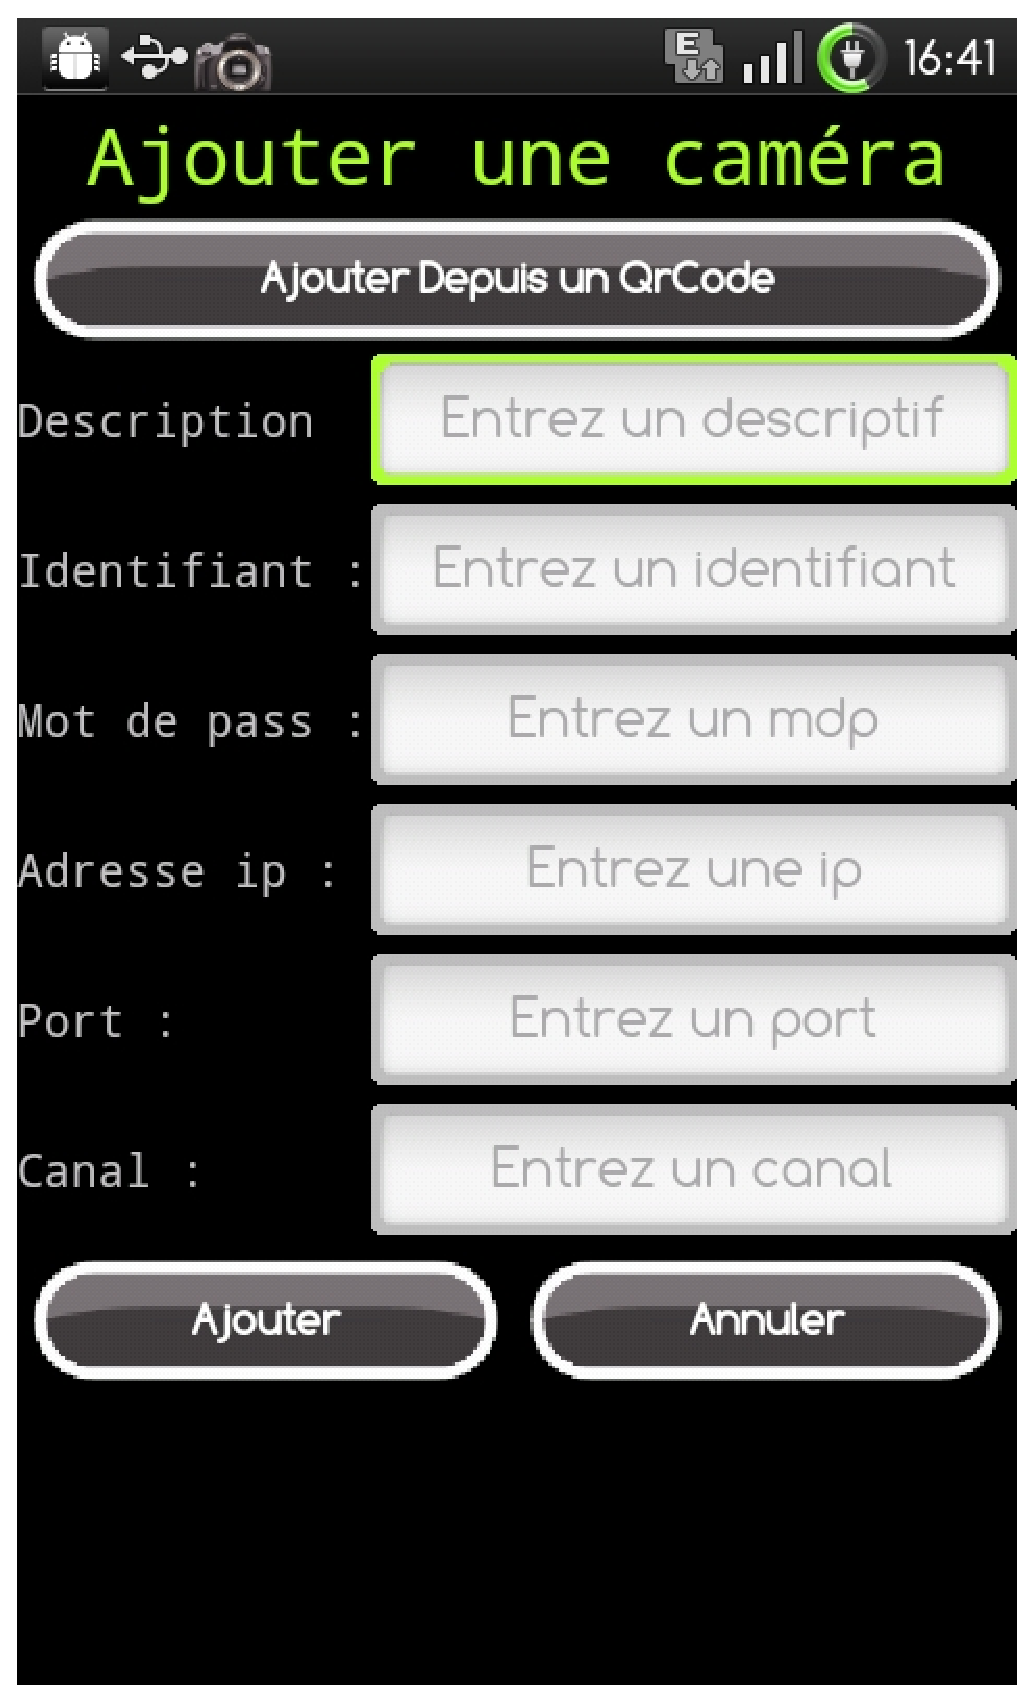
\includegraphics[scale=0.3]{Images/addCamScreenShot.eps}
  \caption{AddCam View SnapShot}
\end{figure}  
\end{center}


On y retrouve des champs de texte édiatable pour chacunes
des caracteristiques de la caméra ainsi qu'un bouton permettant l'ajout de caméra via
\textit{QrCode}.
\indent Le lecteur de code Qr est implémenté par la bibliothèque
\textit{zxing}\footnote{\label{zxing} http://code.google.com/p/zxing/}. \newline
Lors d'un clic sur ce bouton, nous appelons l'activité 
\textit{SCAN} de la bibliotheque zxing avec comme argument
\textit{QR\_CODE\_MODE}.\newline
Si la bibliothèque n'est pas disponible sur l'appareil, nous faisons appel a
\textit{l'android market} afin de telecharger l'application \textit{zxing} (qui
implémente l'ensemble des fonctions proposées par la bibliothèque).
\newpage
\begin{lstlisting}[caption={Lancement de l'activité zxing ou de l'android
market.}] 
    public void onClick(View v) { try {
            Intent intent = new Intent(
                "com.google.zxing.client.android.SCAN");
            intent.putExtra("SCAN_MODE", "QR_CODE_MODE");
            startActivityForResult(intent, 0);
        } catch (ActivityNotFoundException e) {
            String marketSearch = "market://details?id=com.google.zxing.client.android";
            Intent updateIntent = new Intent(Intent.ACTION_VIEW, Uri.parse(marketSearch));
            startActivity(updateIntent);
        }
    }
\end{lstlisting}

\indent \newline
\indent Lorsque l'activitée \textit{zxing} se termine, l'activité
\textit{addCam} recupere l'adresse de la caméra contenu dans le code Qr puis verrouille les
champs de texte édiatable adresse et port.\\
\indent Pour ajouter la nouvelle
caméra, il ne reste plus  é l'utilisateur qu'é cliquer sur le bouton
\textit{ajouter} pour revenir sur l'écran d'acceuil et constater l'ajout de la caméra. Cependant il reste possible de revenir é l'écran d'acceuil sans sauvegarder les changement en cliquant sur \textit{fermer}.

\subsection{Affichage des Caméras}
Une fois la phase de création reussie, nous avons implémenté une nouvelle
activité permettant d'afficher l'ensemble des caméras ajouter par l'utilisateur.
Cette activité s'appele \textit{Home} et est contenue dans la classe
\textit{Home.java}.\newline
Android defini une cycle de vie pour chaque activitée selon le diagramme
decrit par la \textit{figure 3.2}.
\newline
\indent Ce cycle de vie nous permet d'initialiser, d'interrompre, ou de detruire
les differentes vues et fonctionnalitées de notre activitée. Dans le cas de
l'activité \textit{Home} (qui est l'activité d'acceuil de notre application), ce cycle se traduit par : 
\begin{itemize}
  \item   \underline{onCreate :} \begin{enumerate}
    \item Allouer les ressources a l'aide du construteur de la classe parent
    (\textit{super.onCreate(savedInstanceState});)
    \item Récuperation des préférences de l'utilisateur via un
    \textit{SharedPreferences} décrit utlétieurement.
    \item Démarrage du service de détéction de mouvement.
    \item Affichage d'un pop-up d'aide et astuces (si l'utilisateur n'a pas
    choisi de le desactiver).
    \item Lecture de la liste des caméras deja enregistré si disponible.
    \item Mise a jour et implémentation des \textit{listeners} de la liste
    affichant les caméras.\newline
  \end{enumerate} 
  \item \underline{ onActivityResult :}\newline Lorsqu'un activitée demarre une
  autre activitée via les \textit{startActivity(intent)} ou
  \textit{startActivityForResult(intent, 1)} celle-ci passe en arrière plan pour
  executer l'activité décrite par l'\textit{intent}. Durant cette état elle peut
  être ``tuée'' par le gestionnaire de tache, ou en attente d'un resultat. C'est pourquoi l'état
  onResume de la \textit{figure 3.1} englobe également l'état
  \textit{onActivityResult}.\newline
  Pour faire appel a l'activité permettant d'ajouter une caméra, l'utilisateur
  doit utiliser le \textit{Menu} (defini dans la classe \textit{Home.java}) puis
  cliquer sur ``Ajouter une caméra''. Cette action lancera l'activitée
  \textit{addCam} et attendra le resultat (la nouvelle caméra).
  \newline Quand l'utilisateur aura cliqué sur le bouton ``Ajouter'' de
  l'activitée \textit{addCam}, celle-ci ce terminera en ayant defini comme
  resultat le code \textit{OK}, et comme valeure \textit{extra} associé au tag
  deini par la variable\textit{ camTag} la caméra
  précédement \textit{serialisée}.\newline Il ne reste plus qu'a la fonction
  \textit{onActivityResult} de deserialisée la caméra, de l'ajouter dans la
  liste de caméras deja ajoutées (appelé \textit{camList}), et pour finir de
  mettre a jour l'affichage.\newline
  
  \item \underline{onDestroy :}\newline
  Afin de ne pas devoir entrer les caméras à chaque demarrage de
  l'application, nous avons choisis de serealiser puis de sauvegarder la liste
  des caméras dans un fichier pour les ajouter automatiquement à chaque
  demarrage. Cette sauvegarde s'effectue juste avant de liberer les ressources
  en surchargant la fonction \textit{onDestroy}. 
  \end{itemize}
  
\begin{center}
\begin{figure}[H]
  \label{activityLifeCycle}
  \centering
  \fbox{
   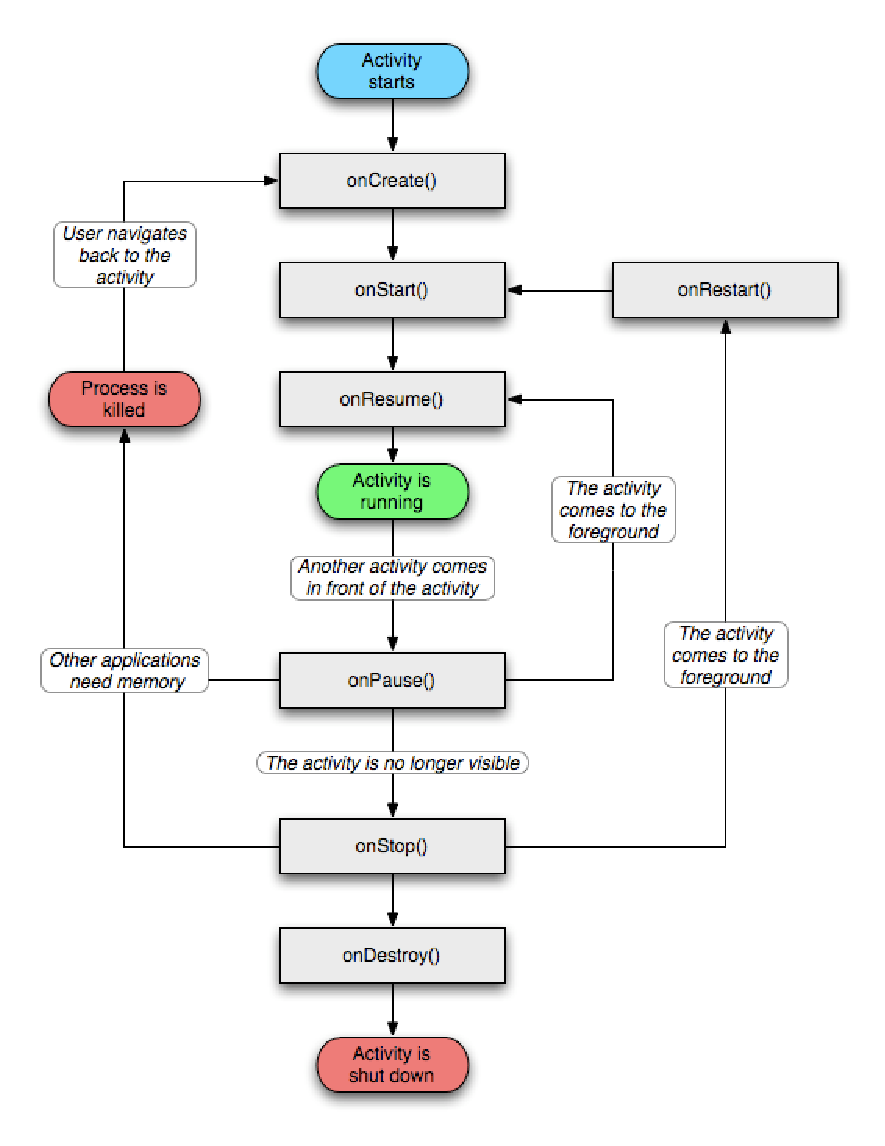
\includegraphics[scale=0.8]{Images/activityLifecycle.eps}
  }
  \caption{Android Activity Life Cycle\protect\footnotemark}
  \end{figure}
  \end{center}
\footnotetext{http://developer.android.com/reference/android/app/Activity.html}
\newpage
 L'affichage de l'activitée \textit{Home} est decris ci-dessous, on peut y
 retrouver une liste personnalisée contenant :
 \begin{itemize}
   \item L'identifiant unique de la caméra.
   \item Suivit de son descriptif.
   \item Puis en indication son l'url.
 \end{itemize}
 On peut également voir en bas de l'image, le menu qui apparait lors de l'appuis
 sur la touche menu du téléphone.\newline
 \begin{center}
 \begin{figure}[H] 
  \label{homeScreenShot}
  \centering
  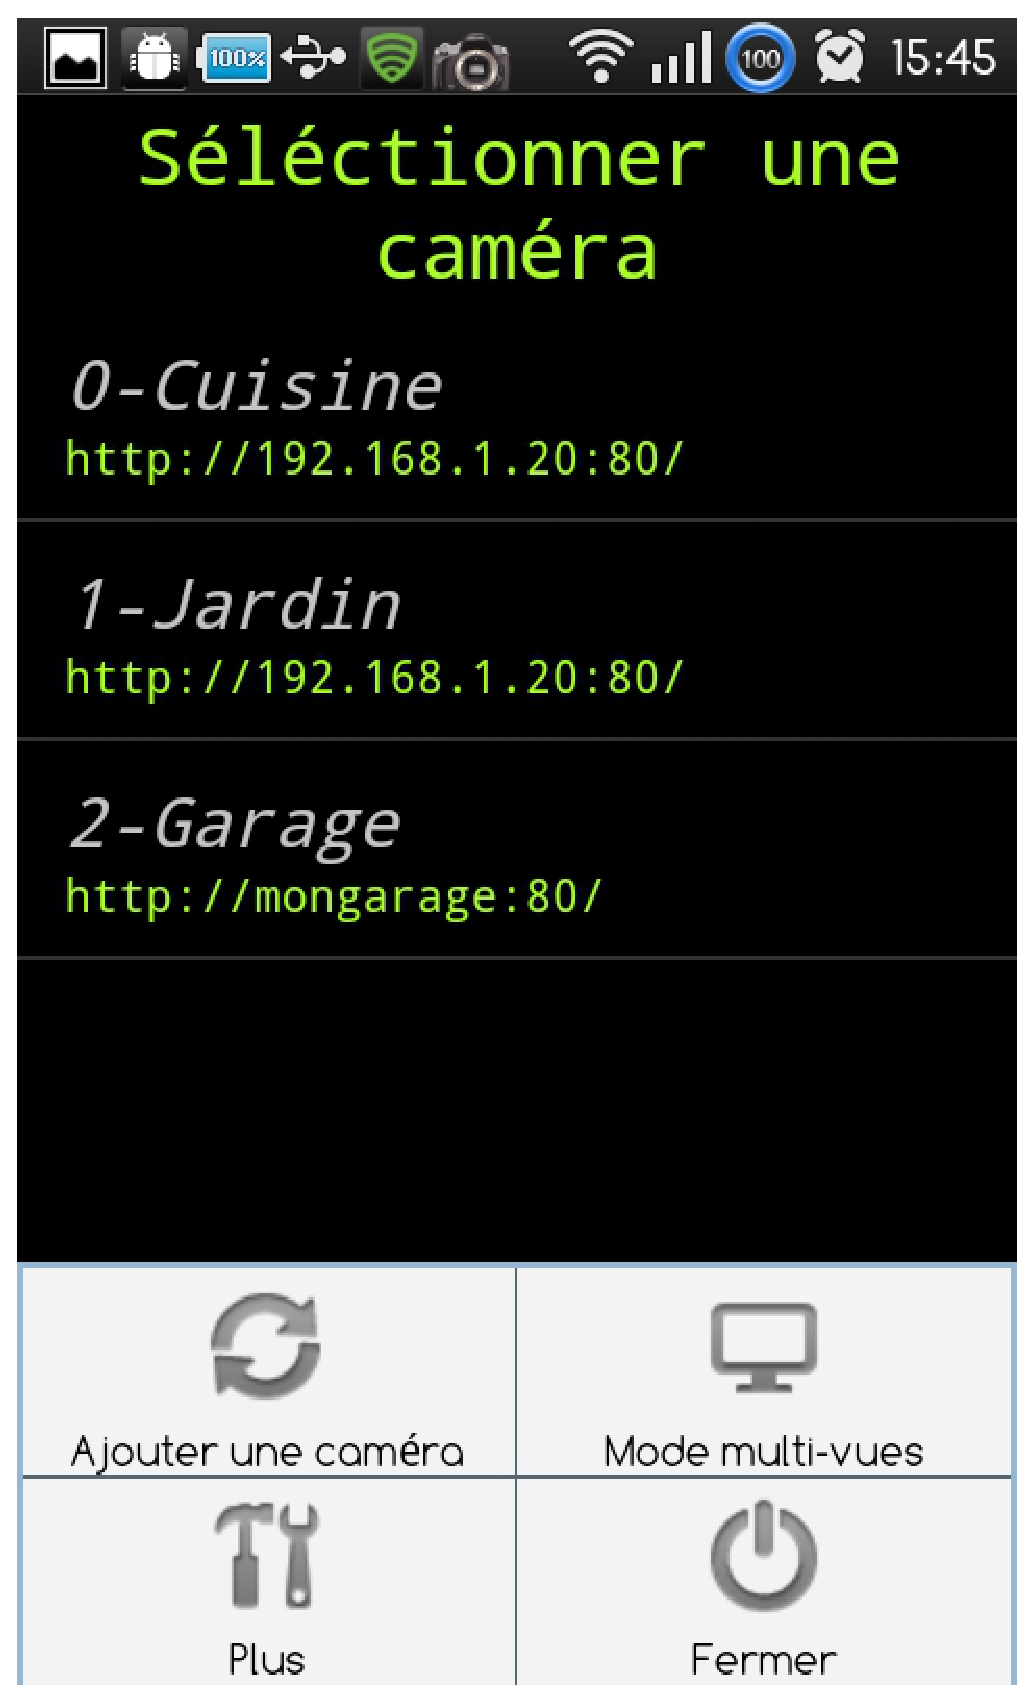
\includegraphics[scale=0.3]{Images/homeScreenShot.eps}
  \caption{Home SnapShot}
\end{figure}  
\end{center}

\subsection{Modification et Suppression de l'objet}
Lors d'un appuis long sur une élément de la liste
(\textit{setOnItemLongClickListener}) une alerte apparait pour demander a
l'utilisateur si il souhaite modifier, ou supprimer l'élément (la caméra).
\begin{itemize}
  \item Si il choisit de supprimer l'élément, une seconde alerte apparait pour confirmer
ou annuler son choix. 
\item Si il choisit de modifier la caméra, l'application lance une nouvelle
activité adaptée a la modification de la caméra. Il peut alors appliquer ou
annuler ses changements sur le meme principe que l'ajout d'une caméra.
\end{itemize}
\newpage
\begin{changemargin}{-1cm}{-1.5cm}
\begin{lstlisting}[caption={Gestion d'un appui long sur un élément de la
liste.}]
public boolean onItemLongClick(AdapterView<?> arg0, 
			View arg1, final int position, long arg3) { 
	AlertDialog alert; 
	AlertDialog.Builder builder = new AlertDialog.Builder(activity);
	builder.setMessage(getString(R.string.messageChoose))
		.setCancelable(false)
		.setPositiveButton(getString(R.string.boutonModifier),
			new DialogInterface.OnClickListener() {
				@Override
				public void onClick(DialogInterface dialog, int id) {
					Intent intent = new Intent(activity.getApplicationContext(),EditCam.class); 
					Bundle objetbunble = new Bundle();
					objetbunble.putSerializable(getString(R.string.camTag),camList.get(position));
					intent.putExtra(getString(R.string.camPosition), position);
					intent.putExtras(objetbunble);
					dialog.cancel();
					startActivityForResult(intent,EDIT_CODE);
		}}).setNegativeButton(getString(R.string.boutonSupprimer),
			new DialogInterface.OnClickListener() {
				@Override
				public void onClick(DialogInterface dialog, int id) {
					removeCam(position);
					dialog.cancel();
		}});
		alert = builder.create();
		alert.show();
		return true;
}});
\end{lstlisting}
\end{changemargin}


\section{Communication avec la caméra}


\section{Gestion du flux vidéo}
\subsection{Vue Simple}
Cette partie consiste a décrire l'implémentation de la retransmission de la
video d'une seul sur le téléphone. On trouve cette implémentation dans la classe
\textit{Video.java} qui implémente l'activitée \textit{Video}.
\subsubsection{Cycle de vie}
Précédement nous avons décrit le cycle de vie de l'activitée \textit{Home}.
Ici nous avons également ajouté des fonctionnalité aux differents états afin de
ne pas consomer de ressource inutilement. En effet, lorsque l'activitée n'est
plus au premier plan, il est inutile de continuer a retransmettre le flux
video.\newline
C'est également le cas pour l'utilisation du verrou nous permettant d'empecher
le telephone de se mettre en veille lors de la retransmission de la video. Le
code suivant illustre l'arret de la video et l'utilisation du verrou
(wl).\newline
Il existe plusieurs type de verrou, pour les utiliser il faut recuperer une
instance du gestionnaire d'énérgie \textit{PowerManager} a l'aide de la
fonction : 
\begin{lstlisting}
 PowerManager pm = Context.getSystemService(Context.POWER_SERVICE).
\end{lstlisting}
Puis demander explicitement la création d'un nouveau verrou
(\textit{PowerManager.WakeLock}) a l'aide de la fonction :
\begin{lstlisting}
 pm.newWakeLock(PowerManager.SCREEN_DIM_WAKE_LOCK,"Tag");
\end{lstlisting}
Ces differents verrou sont definit par le premier argument. Il existe quatre
type de verrou dont les caracteristiques sont definie ci-dessous :\newline
\begin{center}
\begin{tabular}{|l|c|c|c|}
\hline
Flag Value & CPU & Screen & Keyboard \\
\hline
PARTIAL\_WAKE\_LOCK & On* & Off & Off \\
SCREEN\_DIM\_WAKE\_LOCK & On & Dim & Off \\ 
SCREEN\_BRIGHT\_WAKE\_LOCK & On & Bright & Off \\
FULL\_WAKE\_LOCK & On & Bright & Bright \\
\hline
\end{tabular}
\newline
\textit{WakeLock flags table\footnote{\label{wakeLockTable}
http://developer.android.com/reference/android/os/PowerManager.html}}
\newline
\end{center}
Nous avons choisi d'utiliser un verrou \textit{SCREEN\_DIM\_WAKE\_LOCK} afin de
garder simplement allumé avec une luminosité au minimum pour ne pas consomer
exessivement la batterie du téléphone.
\newpage
 \begin{lstlisting}[caption={Video life-cycle}] 
/**
 * Called when Activity start
 */
public void onCreate(Bundle savedInstanceState) {
	super.onCreate(savedInstanceState);
	setContentView(R.layout.video);
	setRequestedOrientation(0);
	
	PowerManager pm = (PowerManager) getSystemService(Context.POWER_SERVICE);
	wl = pm.newWakeLock(PowerManager.SCREEN_DIM_WAKE_LOCK, "My Tags");
	(...)
}
/**
 * Resume video and acquire wakelock when activity resume.
 */
public void onResume() {
	super.onResume();
	wl.acquire();
	if (pause) {
	    mv.resumePlayback();
	    pause = false;
	}
}
 /**
 * Stop video and release wakelock when activity sleep
 */
public void onPause() {
	pause = true;
	wl.release();
	if (mv != null)
	    mv.stopPlayback();
	super.onPause();
}

/**
 * Stop Video before destroy
 */
public void onDestroy() {
	if (mv != null)
	    mv.stopPlayback();
	super.onDestroy();
}
\end{lstlisting}
\subsubsection{ConnectivityManager}
L'accés a internet pour un téléphone disposant d'un systeme d'exploitation
comme Android se fait par des couches phisique de nature differente . Le debit
est donc phortement dependand du support utilisé, c'est pourquoi nous faisons
appel a la classe \textit{ConnectivityManager} afin de récupéré la nature du
support pour definir la resolution aupres de la caméra de la video à envoyer.
Nous avons principalement distingué deux type de réseau : \textit{WiFi} et les
autres réseaux mobile (\textit{3G}, \textit{3G+}, \textit{EDGE}, \ldots).
Afin de definir la correspondance suivant qui nous permet d'obtenir un
taux de raffraichissement correct en \textit{WiFi} (moyenne de 25fps pour une
couverture total) et utilisant la resolution minimal pour les autres reseaux:
\begin{center}
\begin{tabular}{|c|c|}
\hline
Network & Resolution \\
\hline
WiFi &320x240\\
Other &168x120\\
\hline
\end{tabular}
\newline\newline
\end{center}
Pour récupéré le type de réseau on fait une nouvelle fois appel a la
fonction :
\begin{lstlisting}
ConnectivityManager mConnectivity = (ConnectivityManager) getSystemService(Context.CONNECTIVITY_SERVICE);
\end{lstlisting}
Puis en récupérant une instance du réseau actif :
\begin{lstlisting}
NetworkInfo info = mConnectivity.getActiveNetworkInfo();
if (info != null && info.isConnected()) {
  int netType = info.getType();
  if (netType == ConnectivityManager.TYPE_WIFI) {
	/*... Code pour un support de type WiFi ...*/
  } else {
	/*... Code pour les autres supports ...*/
  }
\end{lstlisting}

\subsubsection{Format Vidéo}
Android est capable d'encoder et de decoder un grand nombre de format audio et
video (cf Android Supported Media Formats\footnote{\label{mediaFormat}
http://developer.android.com/guide/appendix/media-formats.html}) a travers
deux protocoles (\textit{HTTP ou RTSP}).\newline
La caméra mise a notre disposition propose uniquement deux formats vidéo :
\textit{MJPEG} via le protocol \textit{HTTP} et \textit{MPEG4} via le protocol
\textit{RTSP}.\newline Cependant malgres que le systeme d'exploitation est
capable d'utiliser le protocole \textit{RTSP}, celui-ci ne nous permet pas de
modifier les requetes afin d'y ajouter l'authentification necessaire pour la
lecture de la video. Celle-ci est donc accessible uniquement si la caméra
autorise les utilisateurs anonyme a la visionner.\newline Nous sommes donc
limité au protocol \textit{HTTP} dans lequel nous avons expliqué précédement
la maniere dont nous nous authentifion.\newline\newline
Nous devons donc utiliser le protocol \textit{HTTP} qui fournit une video au
format \textit{MJPEG}. Ce format n'etant pas géré par le
\textit{mediaPlayer}\footnote{\label{mediaPlayer}
http://developer.android.com/reference/android/media/MediaPlayer.html}, nous
avons du trouver un autre moyen d'afficher la video.
\subsubsection{MjpegView}
Grace a la documentation de la caméra\footnote{\label{docAxis}
http://www.axis.com/techsup/cam\_servers/dev/cam\_http\_api\_2.php} on peut
constater que la vidéo est en realité composé de la succession d'une multitude
d'image. Pour afficher la vidéo il faut donc simplement faire defiler chacune
des images recupéré dans la réponse d'une requete de video \textit{MJPEG}.
\newline
Nous avons trouvé sur internet une composant graphique \textit{OpenSource}
appelé \textit{MjpegView}\footnote{\label{MjpegView}
http://www.anddev.org/multimedia-problems-f28/mjpeg-on-android-anyone-t1871-30.html}
réalisant exactement ce traitement.
Nous avons tout de meme du effectuer quelques modifiaction pour l'adapter a
notre utilisation (comme l'ajout d'une fonction \textit{resumePlayback} pour
redemarrer la lecture de la vidéo par exemple).\newline
Comme chacun des composants graphique, il peut etre ajouter dans une activité ou
defini directement dans une vue au format \textit{xml}.\newline
\begin{center}
\begin{lstlisting}[language=XML, caption={video.xml}]
<de.mjpegsample.MjpegView.MjpegView
	android:id="@+id/surfaceView1"
	android:layout_width="fill_parent"
	android:layout_height="fill_parent" />
\end{lstlisting}
\end{center}
\begin{center}
\begin{lstlisting}[caption={mjpegViewer.java}] 
public void onCreate(Bundle icicle) {
	super.onCreate(icicle);
	MjpegView mv = new MjpegView(this);
	setContentView(mv);
	mv.setSource(URL);
	mv.setDisplayMode(MjpegView.SIZE_BEST_FIT);
	mv.showFps(true);
	(...)
}
\end{lstlisting}
\end{center}


\subsubsection{Interface de controle de la camera}
Nous avons choisi de mettre à disposition les commandes permettant le controle
de la caméra dans cette activité. Ainsi l'utilisateur peur observer instantannément les
modifications.\newline\newline
\indent Le \textit{LayoutInflater} est une service du systeme d'exploitation qui
permet de charger une vue a partir d'un fichier \textit{.xml}. Nous allons utiliser ce
service pour ajouter, ou supprimer un ensemble de composant graphique a la vue
retransmettant la video.
\begin{lstlisting}[caption={LayoutInflater utilisation}]
RelativeLayout screen = (RelativeLayout) findViewById(R.id.RelativeLayout01);
LayoutInflater inflater = (LayoutInflater) getSystemService(Context.LAYOUT_INFLATER_SERVICE);
/* Add view from mds_video.xml */
inflater.inflate(R.layout.mds_video, screen, true);
/* Remove all component contained in the mainLayout */
screen.removeView(findViewById(R.id.mainLayout));
\end{lstlisting}
Voici les differentes vue produitent :

\begin{center}
\begin{figure}[H] 
  \label{videoView}
    \centering
   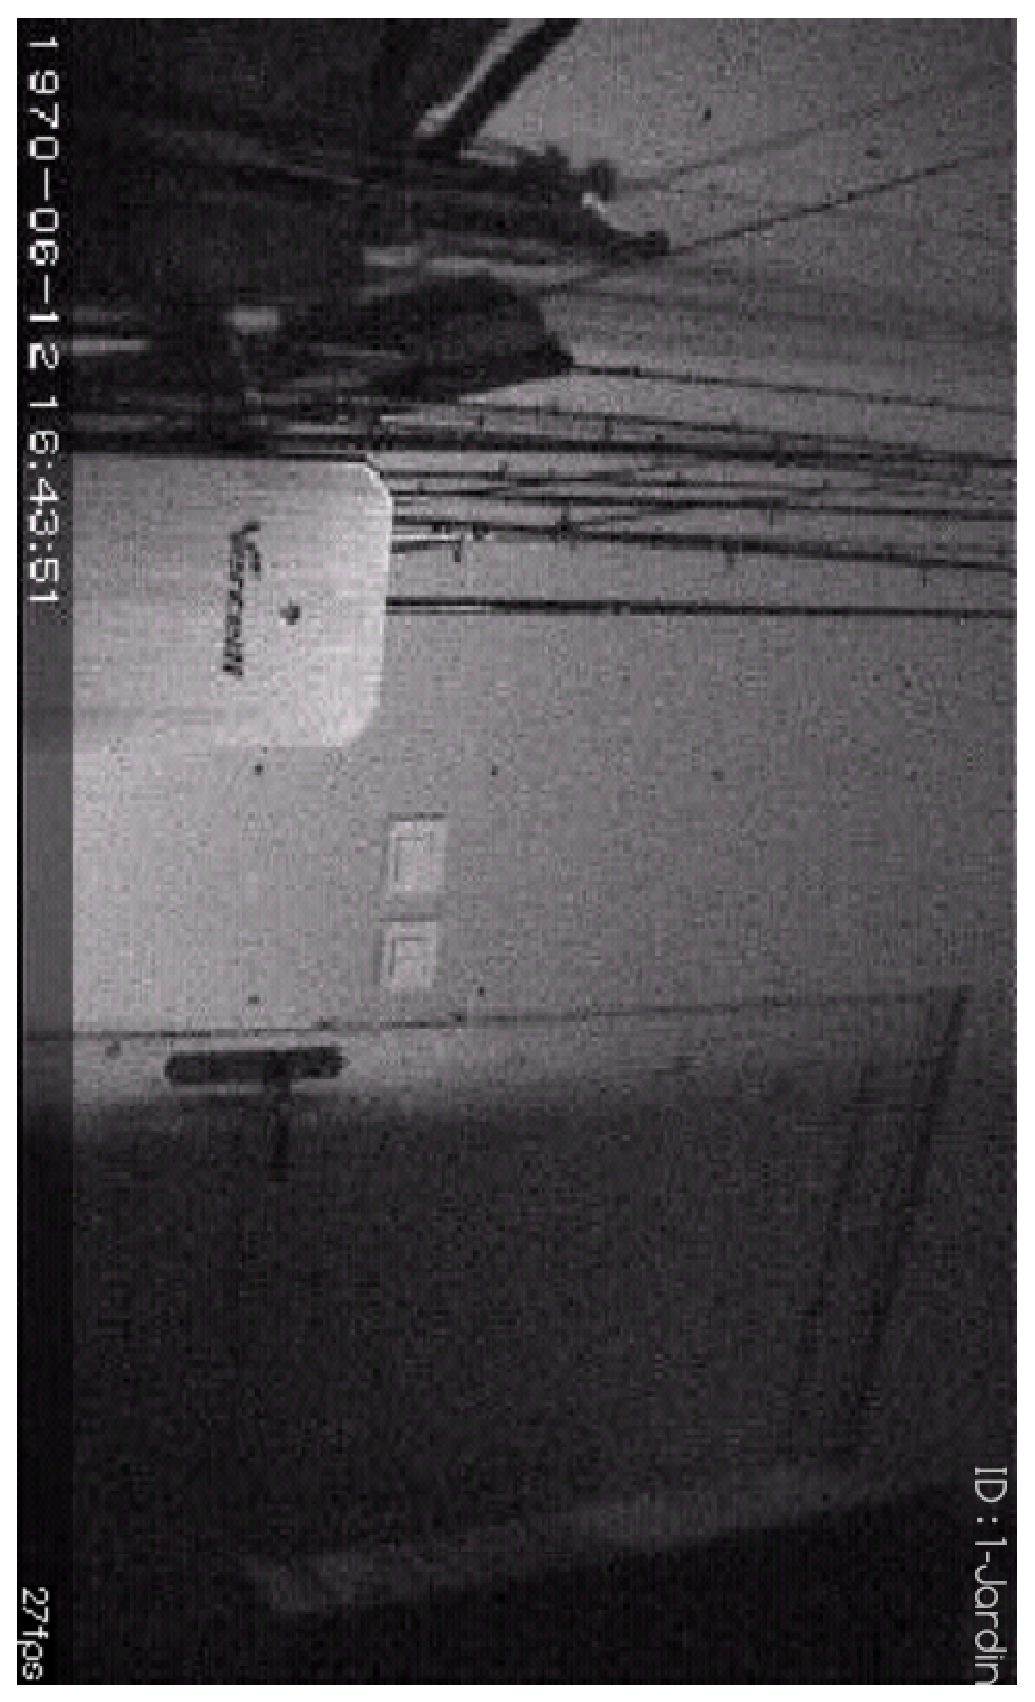
\includegraphics[angle=90,scale=0.3]{Images/videoView.eps}
  \caption{Minimal view for control video.}
\end{figure}
  
\begin{figure}[H] 
  \label{videoViewAdvC}
    \centering
   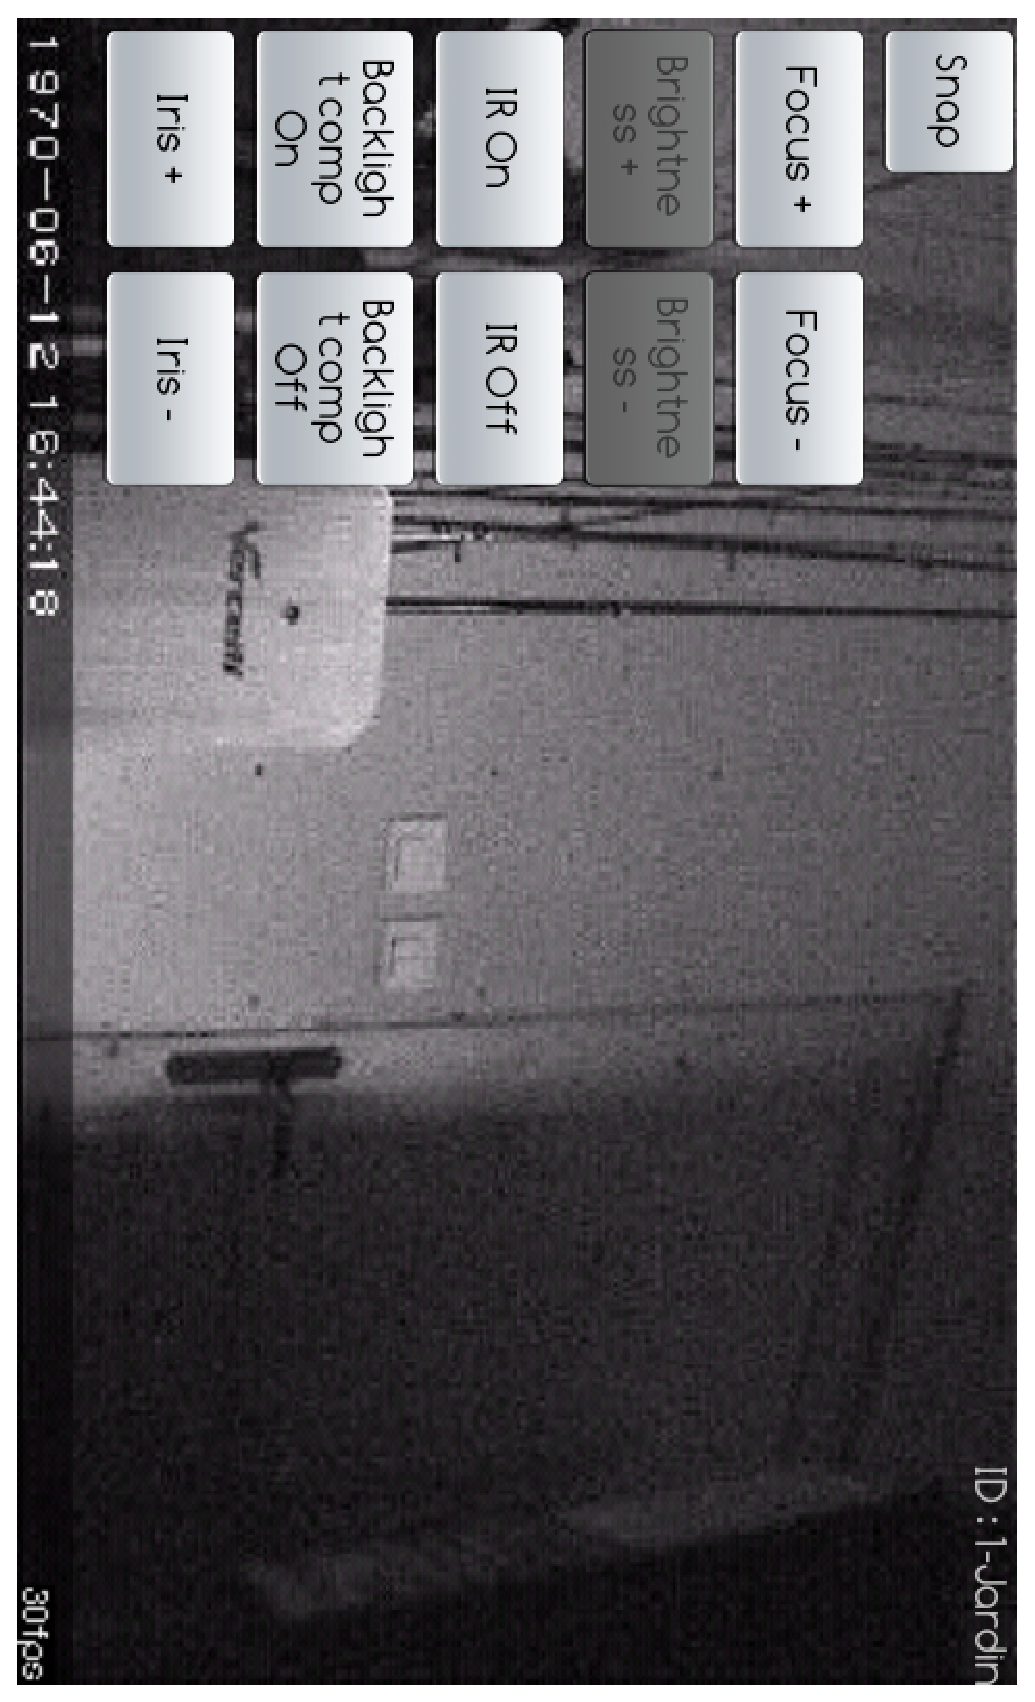
\includegraphics[angle=90,scale=0.3]{Images/videoViewAdvC.eps}
  \caption{Adding components contained in the file \textit{adv\_video.xml}.}
\end{figure}

\begin{figure}[H] 
  \label{videoViewMD}
  \centering
   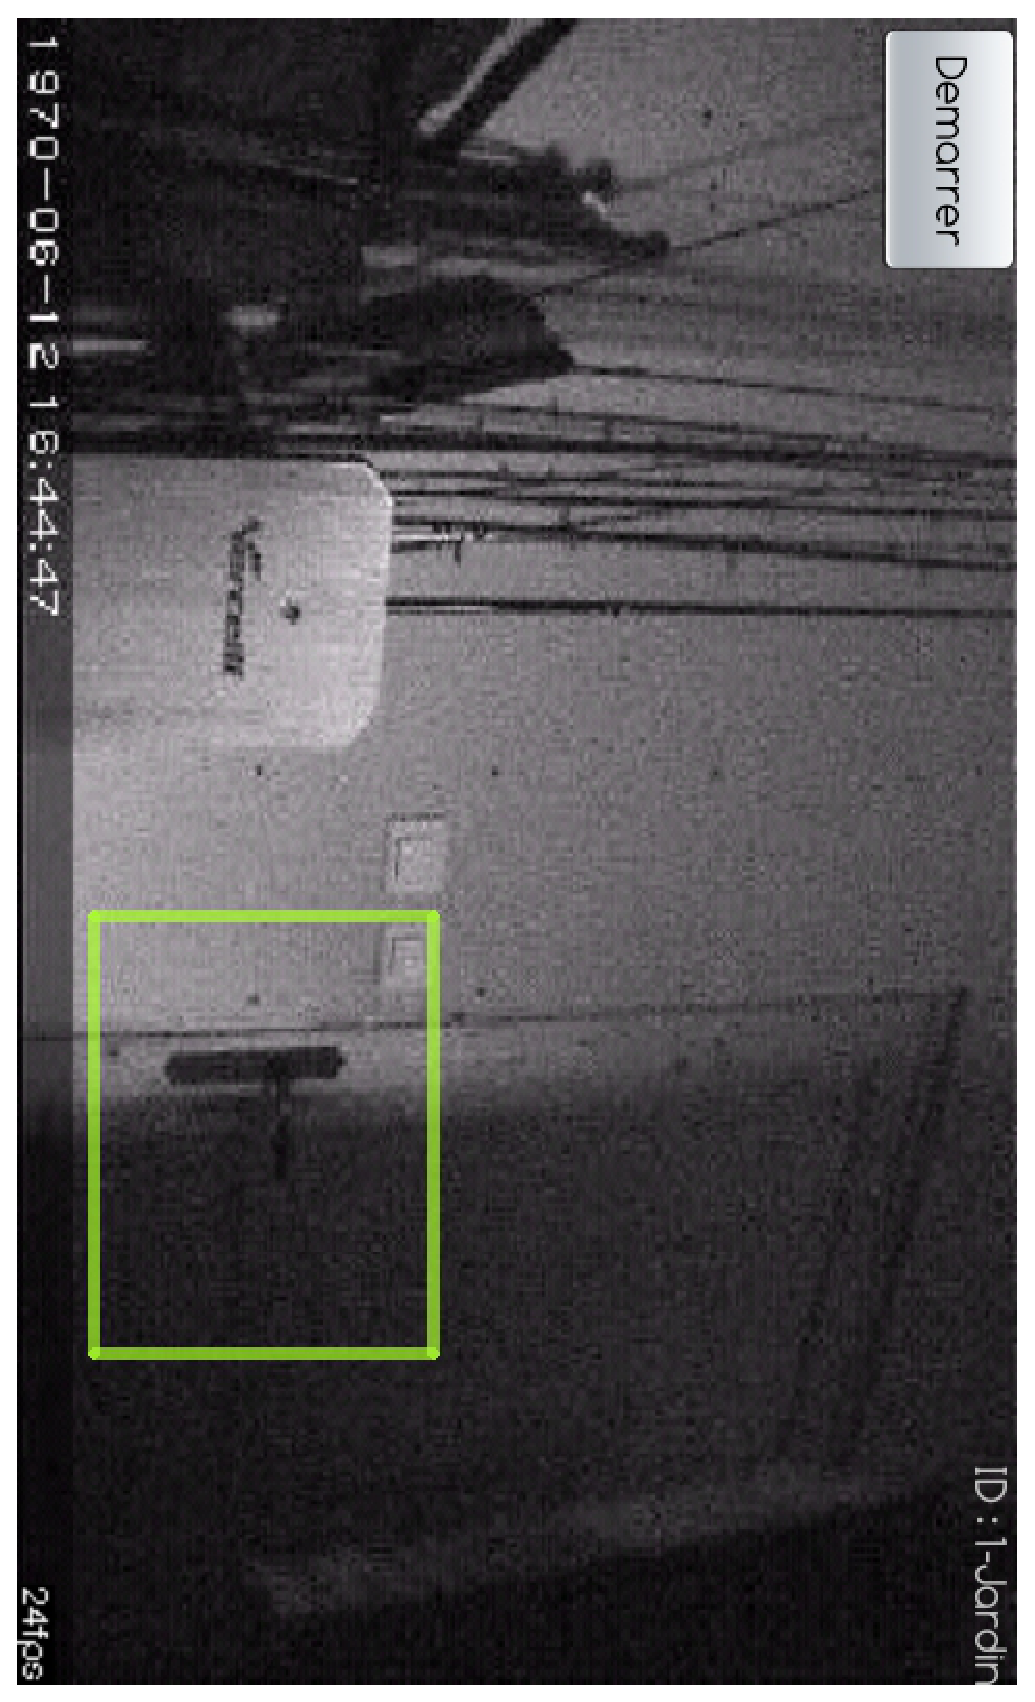
\includegraphics[angle=90,scale=0.3]{Images/videoViewMD.eps}
  \caption{Adding components contained in the file \textit{mds\_video.xml}}
\end{figure}  
\end{center}

Toutes ces vues peuvent etre ajouter ou supprimer en utilisant le menu
personalisé dans l'activitée \textit{Video}.

\subsection{Multi-Vue}
Nous avons souhaité implémenter la possibilitée de visionner plusieurs caméra
simultanement sur une même vue. De nouvelles contraintes sont donc apparuent : 
\begin{itemize}
  \item Comment télécharger et afficher plusieurs vidéos \textit{mjpeg}
  provenant de differentes sources ?
  \item Pouvoir choisir le nombre de caméras à afficher.
  \item Comment choisir les caméras ?
  \item Comment controler les caméras ?
\end{itemize}

\subsubsection{Playerthread video}
Le thread lancé au démarrage d'une activité est appelé \textit{UI Thread}\footnote{\label{UIThread}
http://davy-leggieri.developpez.com/tutoriels/android/ui-thread/} ou
\textit{User Interface thread}. Le role de se thread est d'éxécuter le cycle de
vie de l'activitée. C'est également lui qui gere les interactions
utilisateurs et l'affichage. Seul l'UI thread peut modifier l'affichage
ou capturer une interaction.\newline 
\indent Pour afficher simultanément plusieurs vidéos, nous devons donc utiliser
plusieurs threads afin d'obtenir un affichage fluide des videos.\newline
Chaque thread aura pour tache de telecharger l'image, puis de signaler a l'UI
qu'une nouvelle image est disponible afin d'actualiser
l'affichage.\newline\newline\indent Il existe plusieurs mecanisme pour effectuer
cette notification.\newline
\begin{itemize}
  \item La premiere methode est d'enfiler un obtjet de type
  Runnable, dans la file d'exectution de l'UI a l'aide de la
  fonction : \newline
  \begin{lstlisting}[caption={Example of use runOnUiThread}]
 runOnUiThread(new Runnable() {
 @Override
 public void run() {
	/* Performed by the UI thread */
	imageView[index].invalide();
  }
});  
  \end{lstlisting}
\item Une autre methode consiste a notifier l'UI a l'aide de
\textit{Message} grace a la mise en place d'un \textit{handler} qui
execute une action pour chaque message recu.\newline
\begin{lstlisting}[caption={Example of message handler}] 
/* Performed by the UI thread */
public static Handler myViewUpdateHandler = new Handler() {
  public void handleMessage(Message msg) {
	if (msg.what == GUIUPDATEIDENTIFIER) {
		/* Uptdate View message */
		imageView[index].invalide();
	}
	if (msg.what == URLERRORIDENTIFIER) {
		/* Other message type */
	}
	super.handleMessage(msg);
}};    
\end{lstlisting}    
\end{itemize}
Le diagramme suivant décrit l'execution de l'activitée \textit{MultiVideo}. A
noter la presence d'un delai entre chaque telechargement d'une nouvelle image.
Ce delai nous permet de ralentir le nombre d'image par seconde dans le but de reduire considerablement la consomation de la bande passsante.
L'utilisateur a la possibilité de regler lui meme ce delay dans le menu des
parametres.
 \begin{figure}[H]
  \label{DiagrammeSequenceMultiView}
  \centering
  \fbox{
   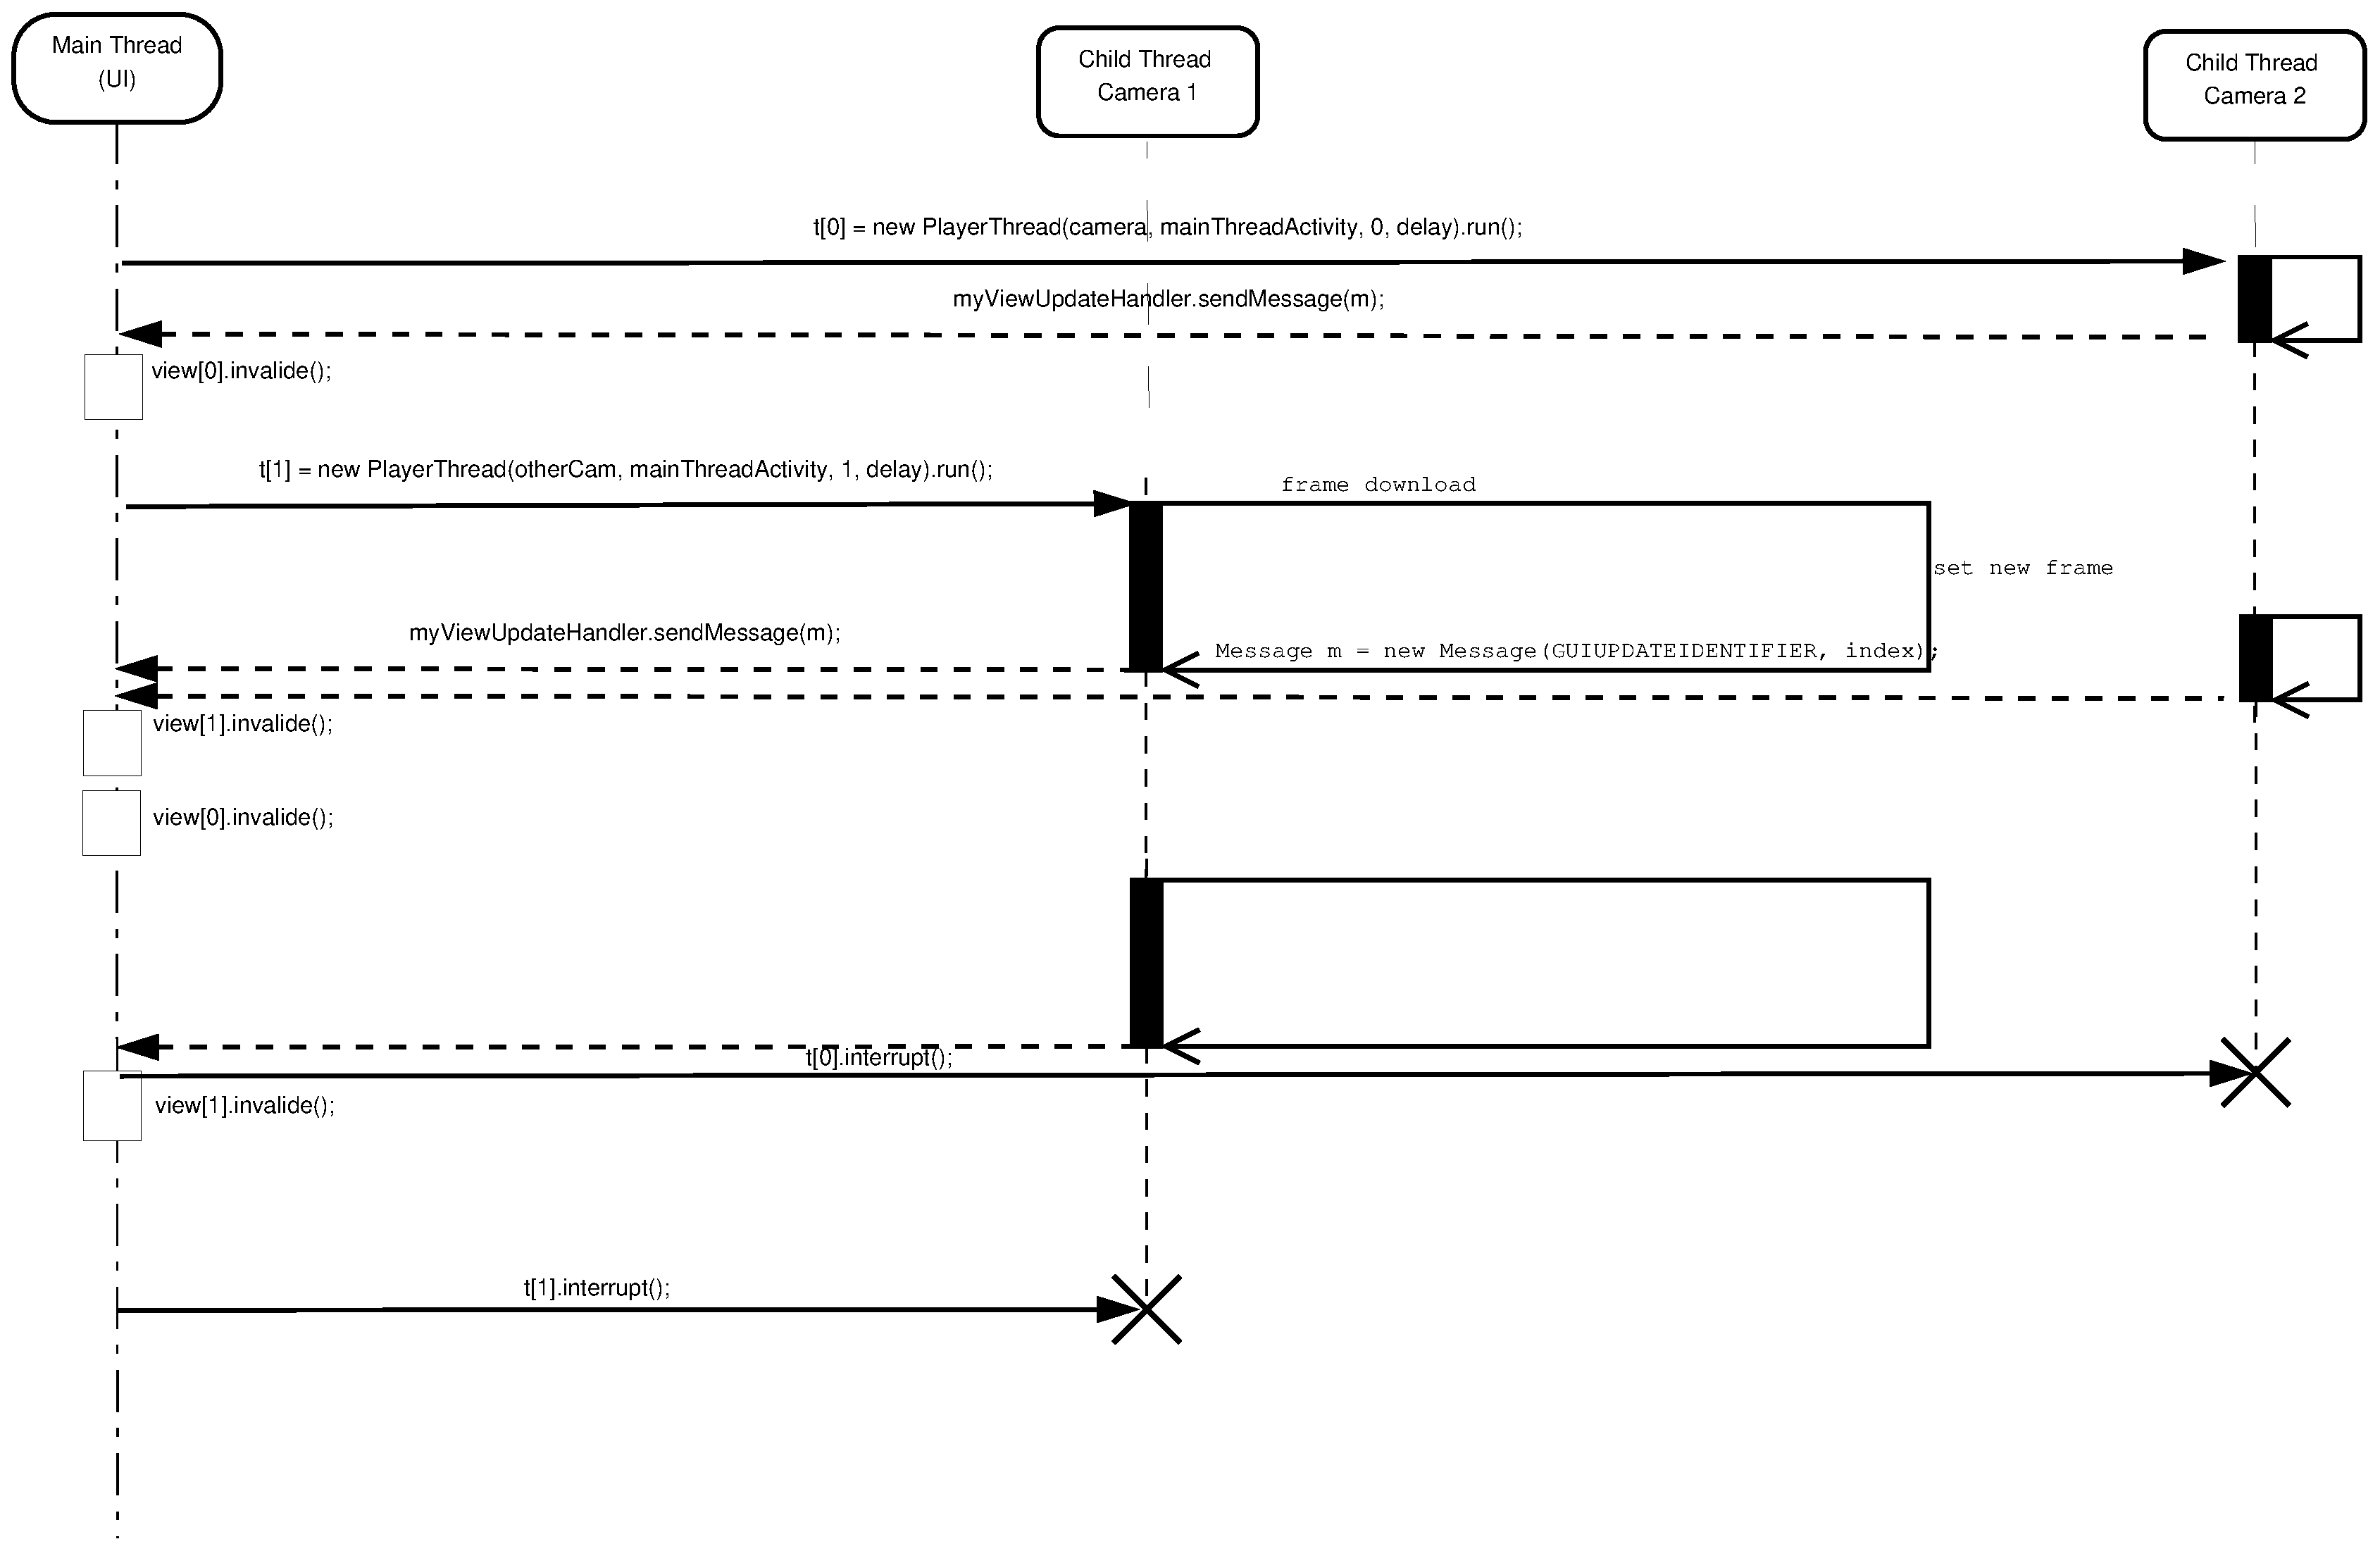
\includegraphics[angle=90,scale=0.4]{Images/DiagrammeSequenceMultiView.eps}
   }
  \caption{Multi-View sequence diagram}
\end{figure}  


\subsubsection{Layout personnalisés}
Maintenant que vous somme capable d'afficher plusieurs video simultanément,
nous nous sommes interessé a la disposition de celles-ci sur l'écran.
Pour sa faire nous offrons dans un premier temps a l'utilisateur la possibilité
de choisir le nombre de caméra a afficher (entre 2 et 6).\newline
Ceci a l'aide d'un alert dialogqui affichera sous forme d'une liste, le nombre
de caméra a afficher. Puis lors de la capture d'un clic sur l'un des element de
la liste, nous lancerons l'activitée \textit{MultiVideo} en y ajoutant un
parametre supplémentaire appelé \textit{nbViewTag} qui definie le nombre de vue
ainsi récupéré.
\begin{changemargin}{0cm}{-2cm}
\begin{lstlisting}[caption={Multi-Video launcher}] 
AlertDialog.Builder builder = new AlertDialog.Builder(activity);
builder.setTitle(getString(R.string.cameraAlertTitle));
builder.setSingleChoiceItems(nb_view, -1, new DialogInterface.OnClickListener(){ 
public void onClick(DialogInterface dialog, int item) {
dialog.dismiss();
Intent intent = new Intent(activity,  MultiVideo.class);
Bundle objetbunble = new Bundle();
objetbunble.putSerializable(getString(R.string.camListTag), camList);
intent.putExtras(objetbunble);
intent.putExtra(getString(R.string.nbViewTag),(item + 2));
startActivity(intent);
}
});
AlertDialog alert = builder.create();
alert.show();
\end{lstlisting}    
\end{changemargin}
Enfin des le lancement de l'activité \textit{MultiVideo}, il ne nous reste plus
qu'a recuperer les parametres pour definir le layout à utiliser.\\
\newline\indent Nous allons maintenant commenter un probleme technique
rencontrer lors de la mise en place des layouts.
Nous avons expliqué precedement la maniere dont nous recupérions le nombre de
caméra a afficher. Afin d'afficher les images recupérées par les differents
threads, nous devons dans un premier temps récépérer chaqunes des adresses des
differentes \textit{ImageView} definie dans les cinq layout. \newline Pour se
faire, toutes les \textit{ImageView} aurons un identifiant defini par leurs
position sur l'ecran :
\begin{itemize}
\item image0 pour le 1er emplacement
\item image1 pour le second
\item image5 pour le 6eme emplacement (le plus grand disponible)
\end{itemize}
En nomant toutes les \textit{ImageView} des differents layout avec un
identifiant equivalent, nous pouvons deduire l'ensemble des adresses en
recupérant celle de l'image0.
En effet lors de la compilation, le compilateur genere un fichier appelé
\textit{R.java}. Dans ce fichier on trouve l'ensemble des adresse pour chaque
classe, layout, et objet de l'application trié par ordre alphabetique. Cette
derniere propriétée nous garantie que l'adresse de l'image1 vaut l'adresse de
l'image0 plus un, etc \ldots. Nous somme donc en mesure de recuperer chacune des 
\textit{ImageView} afin de les mettres a jours, lors de la reception de nouvelle
images mais aussi de definir les \textit{listener} pour capturer les
interactions.
\begin{changemargin}{0cm}{-2cm}
\begin{lstlisting}[caption={ImageView address resolver}] 
/*
 * get R.id.image0 address and inc it to find R.id.image1,
 * R.id.image2, ... , R.id.image.n
 */
int dep = R.id.image0;
for (int i = 0; i < nbView; i++) {
img[i] = (ImageView) findViewById(dep + i);
/* Set Image and Listener for each view */
camView[i] = null;
img[i].setImageResource(R.drawable.cadre);
img[i].setOnClickListener(new myOnClickListener(i));
img[i].setOnLongClickListener(new myOnLongClickListener(i));
}
\end{lstlisting}   
\end{changemargin}

 \begin{figure}[H]
  \label{2cam.eps}
  \centering
   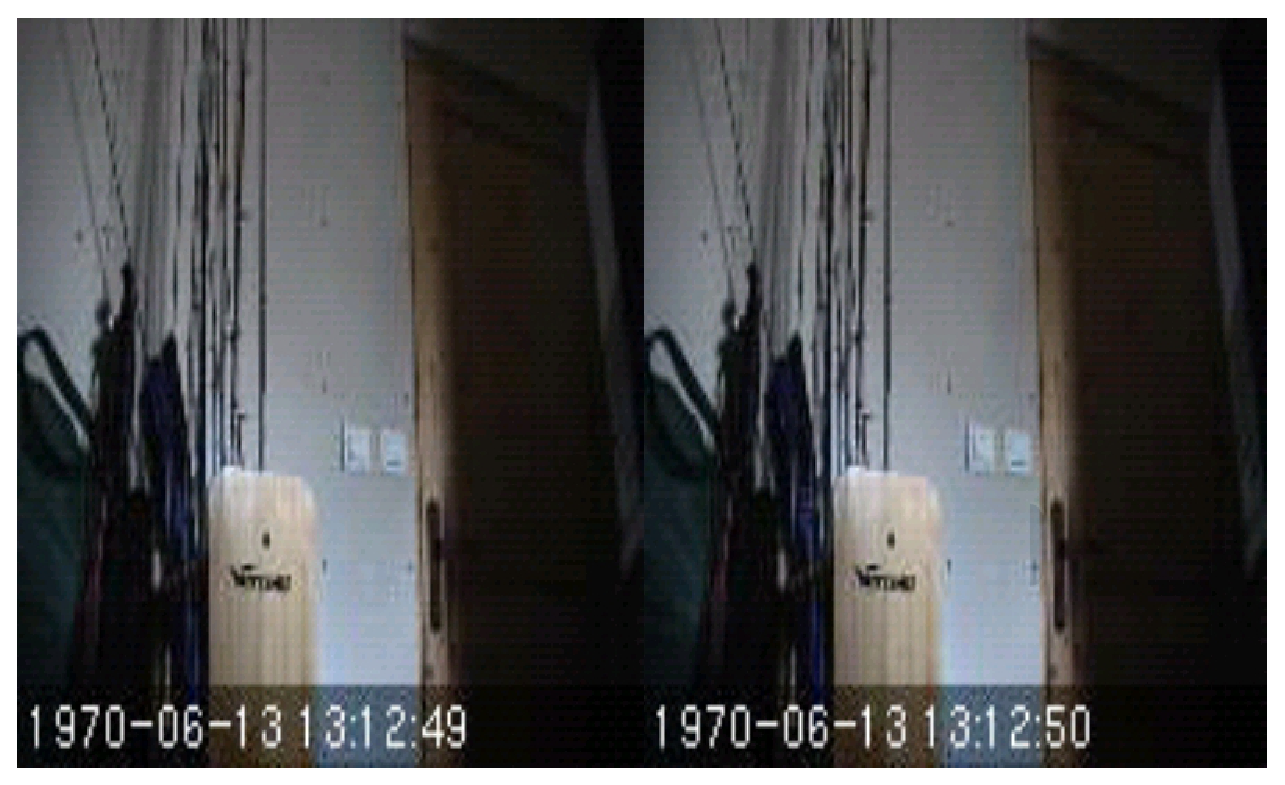
\includegraphics[scale=0.4]{Images/2cam.eps}
  \caption{Multi-View 2 camera}
\end{figure}  
\begin{figure}[H]
  \label{3cam.eps}
  \centering
   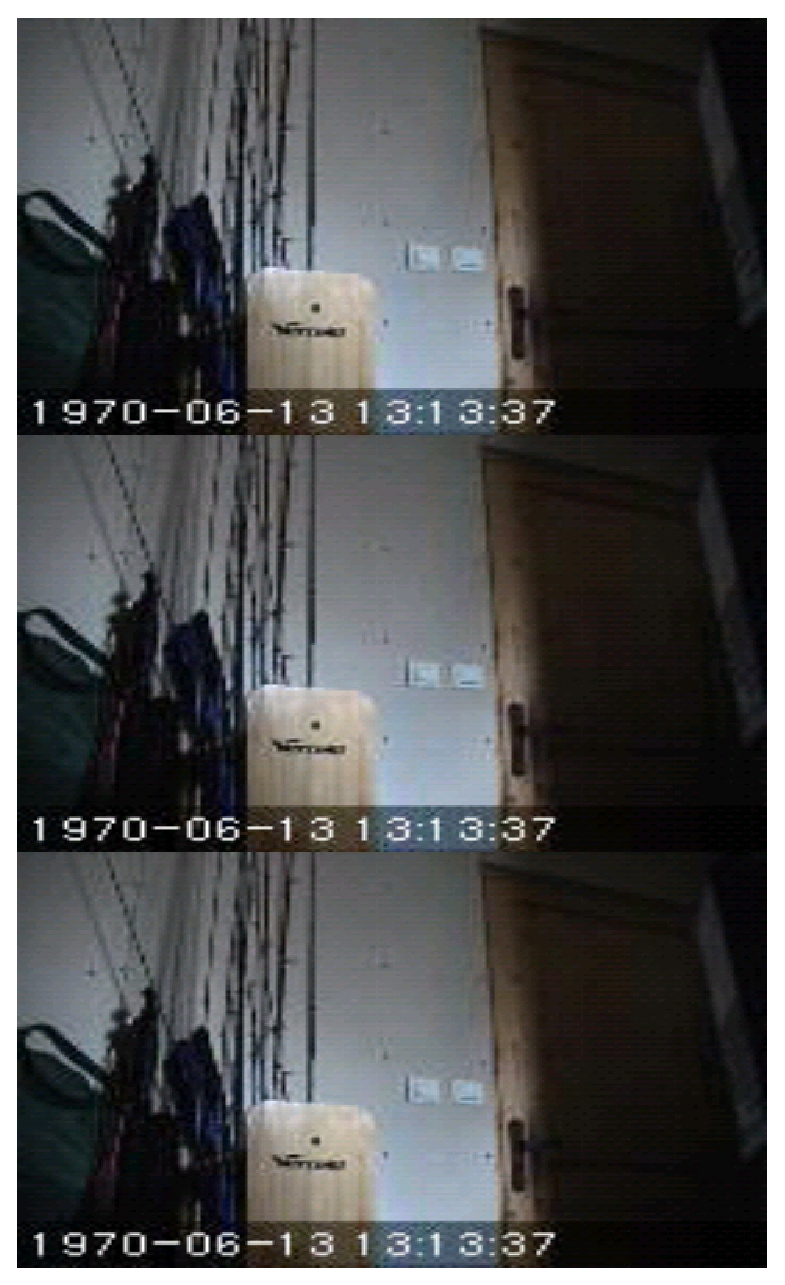
\includegraphics[scale=0.4]{Images/3cam.eps}
  \caption{Multi-View sequence 3 camera}
\end{figure}  
\begin{figure}[H]
  \label{5cam.eps}
  \centering
   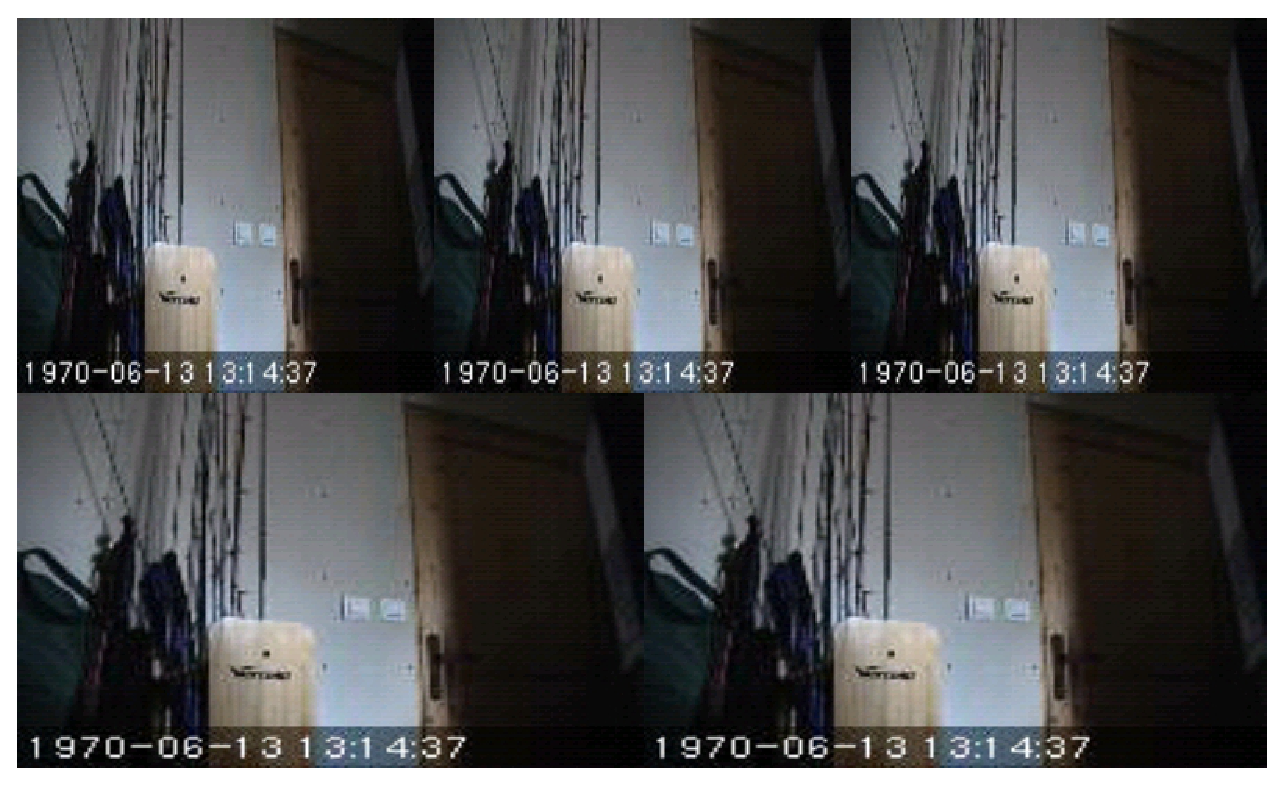
\includegraphics[scale=0.4]{Images/5cam.eps}
  \caption{Multi-View 5 camera}
\end{figure}  
\subsubsection{Utilisation}
Nous offrons a l'utilisateur de choisir la caméra a afficher sur chacune des
\textit{ImageView}. 
\begin{itemize}
\item Le premier clique sur l'une d'elle affiche une liste permettant de
choisir la caméra a afficher.
\item Un nouveau clique stop la vidéo.
\item Un long clique lance l'activitée \textit{Video} pour donner a
l'utilisateur de controler la caméra. Une fois les reglages effectuer, il peut
revenir sur la vue precedent en appuyant sur le bouton retour de son telephone.
\end{itemize}

\section{Contrôle de la caméra}
\subsection{CameraControl}
La communication pour le contrôle du Pan/Tilt/Zoom et des fonctionnalités spécifiques (snapshot, contrôles avancés) de la caméra s'effectuent à travers la classe \textit{CameraControl}.
Les fonctions \textit{changeValFunc} et \textit{switchAutoFunc} permettent d'envoyer les requêtes HTTP à la caméra pour changer la valeur des différents paramètres de celle-ci :
- \textit{PAN}, \textit{TILT}, \textit{FOCUS}, \textit{IRIS}, \textit{BRIGHTNESS} identifient des paramètres prenant une valeur flottante
- \textit{AUTOFOCUS}, \textit{AUTOIRIS}, \textit{AUTO\_IR}, \textit{BACKLIGHT}
identifient des paramètres dont la valeur est comprise dans { \textit{on}, \textit{off}, \textit{auto} } Une réponse HTTP de code \textit{HttpURLConnection.HTTP\_NO\_CONTENT} (code 204)
indique la réussite de la requête, cependant nous ne savons pas si l'action a bien été effectuée.

La fonction \textit{takeSnapshot} réalise la requête de capture d'écran avec comme résolution la valeur passée en paramètre.
Elle retourne les données renvoyées par la caméra sous forme d'un objet \textit{Bitmap}.

Cette classe s'occupe également des activation/désactivation de la détection :
\begin{itemize}
	\item \textit{addMotionD} ajoute une fenêtre de détection.
	\item \textit{removeMotionD} supprime une fenêtre de détection existante.
	\item \textit{updateMotionDParam} met à jour certains paramètres de la fenêtre
	de détection comme les coordonnées ou la sensibilité de détection.
\end{itemize}

Lors du chargement du menu et du layout des contrôles avancés de la caméra, nous vérifions si les fonctionnalités correspondantes sont supportées et/ou activées à l'aide des fonctions
\textit{isSupported} et \textit{isEnabled}. Un appui sur les boutons du menu (celui-ci apparaissant lors de l'appui sur la touche "Menu") déclenchera une alerte texte si la fonctionnalité n'est pas
disponible, alors que pour le layout des contrôles avancés nous définissons la disponibilité de la fonctionnalité directement par l'état du bouton (activé/désactivé).

\subsection{TouchListener}
Le contrôle du PTZ tactile a été implémenté à l'aide de la classe \textit{TouchListener}. Nous avons défini deux gestes possibles avec un ou plusieurs pointeurs (doigt, stylet, ...) pour notre application :
\begin{itemize}
\item un déplacement avec un seul pointeur pour faire bouger la caméra (Pan/Tilt)
\item un écartement/rapprochement de deux pointeurs pour zoomer/dézoomer
\end{itemize}
Cette classe implémente l'interface \textit{OnTouchListener} fournissant une fonction \textit{onTouch} dans laquelle nous gérons chaque mouvement du ou des pointeurs à partir d'un objet \textit{MotionEvent}. Un geste sous Android est défini par une suite de mouvements de type \textit{MotionEvent}.
Il existe une dizaine de types d'actions possibles pour \textit{MotionEvent}, cependant nous utilisons seulement les 4 suivants pour notre application :
\begin{itemize}
\item \textit{ACTION\_DOWN} : le premier pointeur a été ajouté (le geste est
commencé) et l'événement contient les coordonnées du pointeur
\item \textit{ACTION\_POINTER\_DOWN} : un nouveau pointeur a été ajouté
\item \textit{ACTION\_POINTER\_UP} : un pointeur a été enlevé
\item \textit{ACTION\_UP} : le dernier pointeur a été enlevé (le geste est
terminé) et l'événement contient les coordonnées du dernier pointeur
\end{itemize}
A partir de ces types d'actions, nous pouvons définir le déplacement de la
caméra par la suite \textit{ACTION\_DOWN - ACTION\_UP} et la gestion du zoom par
la suite : \\ \textit{ACTION\_DOWN - ACTION\_POINTER\_DOWN - ACTION\_DOWN\_UP -
ACTION\_UP} (nous considérons cependant que le zoom n'est réalisé qu'à partir de l'événement
\textit{ACTION\_POINTER\_DOWN}).

Le champ \textit{mode} contient l'état actuel du geste, soit une des constantes \textit{NONE}, \textit{DRAG} ou \textit{ZOOM}.
Nous récupérons également les dimensions de la vue par \textit{getWidth} et \textit{getHeight} pour la mise à l'échelle des distances de déplacements. 
Pour représenter les coordonnées des pointeurs, nous avons utilisé le type \textit{PointF}.

Nous avons implémenté dans cette classe des méthodes de calcul géométrique entre deux objets \textit{PointF} :
\begin{itemize}
	\item \textit{calculateMoveX} pour la différence en abscisse.
	\item \textit{calculateMoveY} pour la différence en ordonnée.
	\item \textit{calculateDistance} pour la distance géométrique.
\end{itemize}

Nous avons également développé des méthodes pour mettre à l'échelle le déplacement des pointeurs sur l'écran par rapport au déplacement réel réalisé par la caméra :
\begin{itemize}
	\item \textit{scaleMoveX} pour le déplacement en abscisse, en utilisant la
	largeur de l'écran \textit{getHeight}.
	\item \textit{scaleMoveY} pour l'échelle en ordonnée, en utilisant la hauteur
	de l'écran \textit{getWidth}.
	\item \textit{scaleZoom} pour le zoom/dézoom, en utilisant \textit{zoomStep}.
\end{itemize}

Afin de rendre moins ``agressif'' le déplacement sur le téléphone, nous avons
mis en place un paramètre de sensibilité, celui-ci étant modifiable dans les préférences.
Le thread est également endormi quelques millisecondes afin d'éviter la
surcharge d'événements à traiter.
Le tableau ci-dessous montre le traitement
réalisé par la méthode \textit{onTouch} dont le code est présenté après.\newline
\begin{table}[H]
\centering
\begin{tabular}{|p{0.2\linewidth}|p{0.4\linewidth}| p{0.4\linewidth}|}
\hline
Type ACTION & Geste du déplacement & Geste du zoom \\
\hline
DOWN & Mise en mémoire des coordonnées du point de départ &  \\
 & \textit{mode = DRAG} & \\
POINTER\_DOWN & & Calcul et mise en mémoire de la distance de départ \\
 & & \textit{mode = ZOOM} \\
POINTER\_UP & & Calcul et mise en mémoire de la distance d'arrivée \\
UP & Calcul des déplacements horizontaux et verticaux & Calcul du ratio entre les deux distances \\
 & Mise à l'échelle des déplacements & Mise à l'échelle du ratio (avec le champ \textit{zoomStep}) \\
 & \textit{mode = NONE} & \textit{mode = NONE} \\
\hline
\end{tabular}
\caption{Algorithme de traitement onTouch}
\end{table}

\begin{lstlisting}
public boolean onTouch(View v, MotionEvent event) {
	width = v.getWidth();
	height = v.getHeight();
	switch (event.getAction() & MotionEvent.ACTION_MASK) {
	case MotionEvent.ACTION_DOWN:
	    current.set(event.getX(), event.getY());
	    mode = DRAG;
	    Log.i(TAG, "mode=DRAG");
	    break;

	case MotionEvent.ACTION_POINTER_DOWN:
	    currentDist = calculateDistance(
		    new PointF(event.getX(0), event.getY(0)),
		    new PointF(event.getX(1), event.getY(1)));
	    mode = ZOOM;
	    Log.i(TAG, "mode=ZOOM");
	    break;

	case MotionEvent.ACTION_POINTER_UP:
	    startDist = currentDist;
	    currentDist = calculateDistance(
		    new PointF(event.getX(0), event.getY(0)),
		    new PointF(event.getX(1), event.getY(1)));
	    Log.i(TAG, "mode=ZOOM(P_UP)");
	    break;

	case MotionEvent.ACTION_UP:
	    if (mode == DRAG) {
		PointF start = new PointF(current.x, current.y);
		current.set(event.getX(), event.getY());
		float moveX = scaleMoveX(calculateMoveX(start, current));
		float moveY = scaleMoveY(calculateMoveY(start, current));
		Log.i(TAG, "move(X,Y):" + moveX + "," + moveY+ "sensibilite / " + sens);
		camC.changeValFunc(CameraControl.PAN, -1* moveX / sens, -1 * moveY
			/ sens);
	    } else if (mode == ZOOM) {
		Log.i(TAG, "startDist=" + startDist);
		Log.i(TAG, "currentDist=" + currentDist);
		if (Math.abs(startDist - currentDist) > 10) {
		    float ratio = (currentDist / startDist > 1) ? currentDist
			    / startDist : -1 * (startDist / currentDist);
		    Log.i(TAG, "ratio=" + ratio);
		    camC.changeValFunc(CameraControl.ZOOM, scaleZoom(ratio), 0);

		}
	    }
	    mode = NONE;
	    Log.i(TAG, "mode=NONE");
	    try {
		/* Bloc UI thread to not spam request */
		Thread.sleep(200);
	    } catch (InterruptedException e) {
		e.printStackTrace();
	    }
	    break;
	}
\end{lstlisting}
\section{Fonctionnalités avancées et réglages}
Les caméras \textit{Axis} offrent un grand nombre de services pour lesquels
nous avons implementer la possibiliter de les utiliser directement avec le
telephone.
\subsection{Snapshot}
Parmis ces services, la camera propose a l'utilisateur la possibilite de
prendre une photo instantanée. \newline
Pour ce faire il nous suffit d'envoyer une requete \textit{HTTP} a l'adresse
suivante : 
\begin{lstlisting}
http://<servername>/axis-cgi/jpg/image.cgi
\end{lstlisting}
Dans cette requete, nous avons la possibilitée d'ajouter de nombreux parametres
comme la résolution, le taux de compression, l'affichage de la date, l'heure,
etc. Toutes ces options sont décritent dans la documentation de la caméra
\footnote{\label{MjpegView}http://www.axis.com/techsup/cam\_servers/dev/cam\_http\_api\_2.php\#api\_blocks\_image\_video\_jpeg\_snapshot}.
L'image est contenu dans la réponse :
\begin{lstlisting}
HTTP/1.0 200 OK\r\n
Content-Type: image/jpeg\r\n
Content-Length: <image size>\r\n
\r\n
<JPEG image data>\r\n
\end{lstlisting}
Une fois la resolution choisi, il ne nous reste qu'a convertir le flux en image
a l'aide de la fonction :
\begin{lstlisting}
Bitmap bmp = BitmapFactory.decodeStream(stream);
\end{lstlisting}
puis l'enregistrer dans un fichier :
\begin{lstlisting}
 bmp.compress(Bitmap.CompressFormat.JPEG, 80, fichier);
\end{lstlisting}
Afin de prévenir l'utilisateur de la reception de la capture, nous avons
implémenté une fonction permettant d'ajouter une notification personnalisée dans
la barre de status du telephone.\newline
En plus de notifier l'utilisateur, nous lui offrons la possibilitée de visionner
la photo en cliquant sur la notification.
\begin{changemargin}{0cm}{-2cm}
\begin{lstlisting}[caption={ImageView address resolver}] 
 public static void statusBarNotificationImage(Activity activity, Bitmap bmp, String text, String path, int id, String tag) {
	NotificationManager notificationManager;
	notificationManager = (NotificationManager) activity.getSystemService(Context.NOTIFICATION_SERVICE);
	Notification notification = new Notification(R.drawable.camera,	"Camera-Axis", System.currentTimeMillis());
	notification.contentView = new RemoteViews(activity.getPackageName(), R.layout.notification);
	/* Notification action (Open gallery) */ 
	Intent intentNotification = new Intent();
	intentNotification.setAction(android.content.Intent.ACTION_VIEW);
	intentNotification.setDataAndType(Uri.fromFile(new File(path)), "image/png");
	PendingIntent pendingIntent = PendingIntent.getActivity(activity.getApplicationContext(), 0, intentNotification, 0);
	notification.defaults |= Notification.DEFAULT_VIBRATE;
	notification.contentIntent = pendingIntent;
	notification.contentView.setImageViewBitmap(R.id.Nimage, bmp);
	notification.contentView.setTextViewText(R.id.Ntext, text);
	notificationManager.notify(tag, id, notification);
    }
\end{lstlisting}   
\end{changemargin}
Ainsi nous obtenons la notification suivante : 
\begin{figure}[H]
  \label{notification}
  \centering
   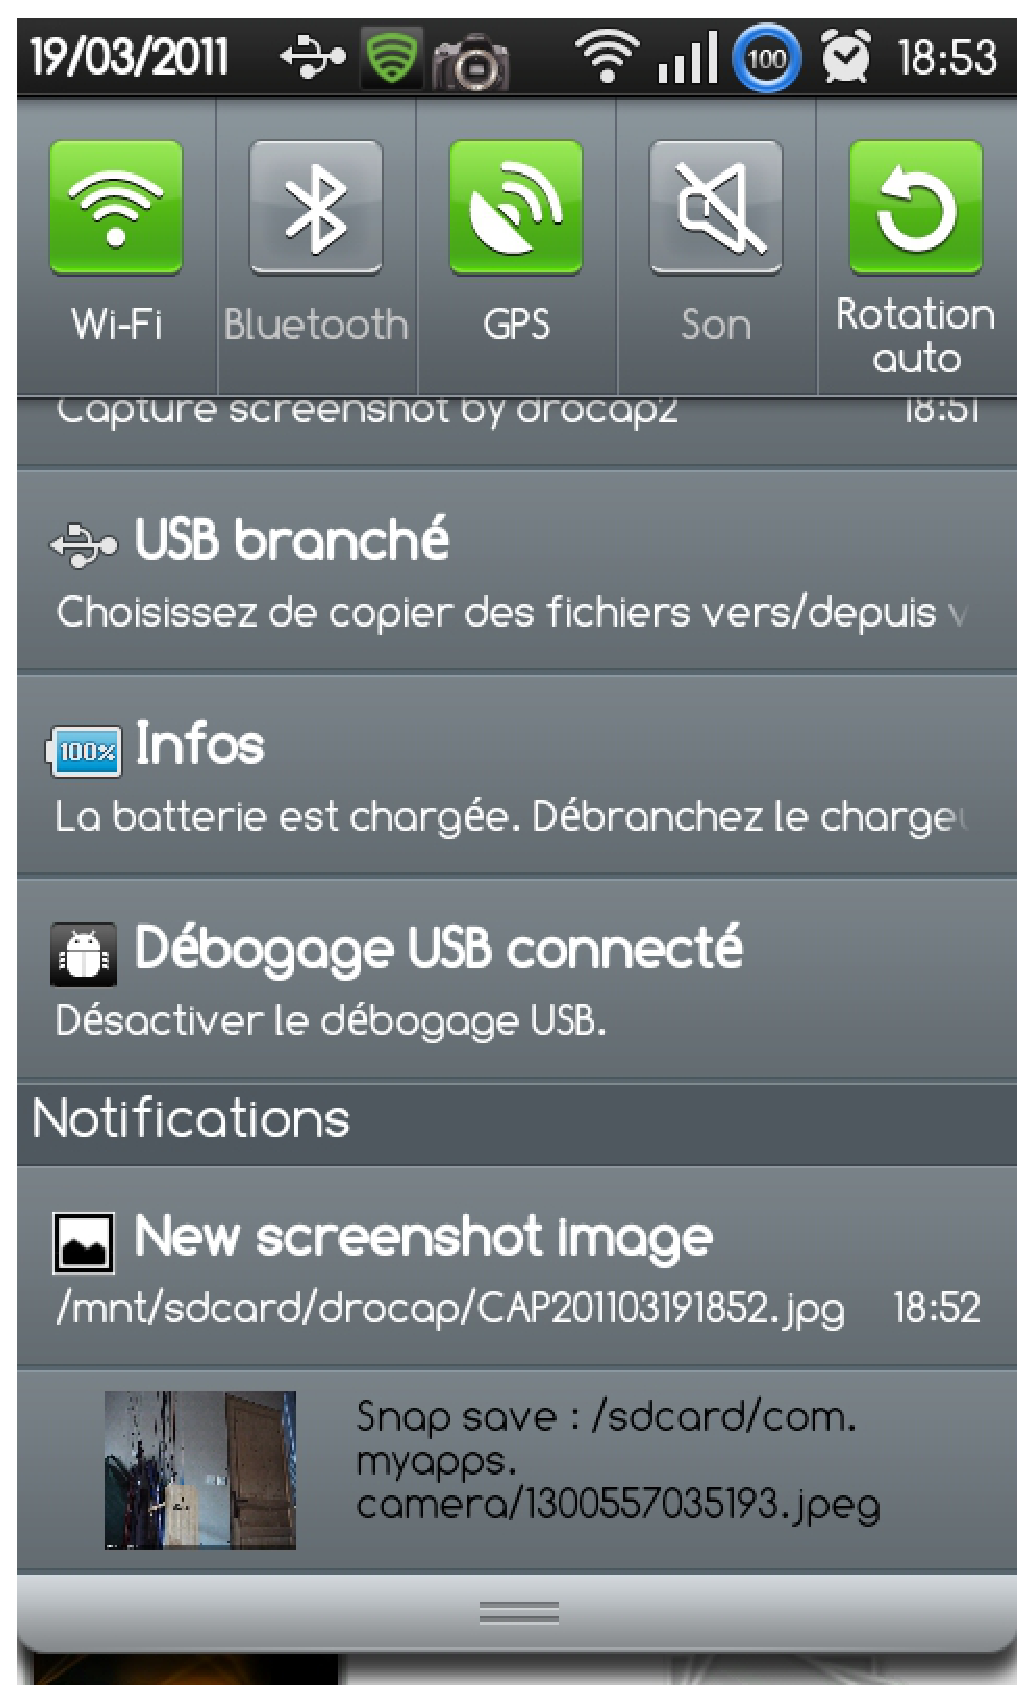
\includegraphics[scale=0.4]{Images/notification.eps}
  \caption{Notification SnapShot}
\end{figure}  

\subsection{Autres réglages}
Afin d'ameliorer la visibilitée de la caméra, celle ci propose un grand nombre
de fonction comme le réglage de la luminositée, de la mise au point
(focus), l'ouverture ou la fermeture de l'iris, et beaucoup d'autres fonctions
egalement disponible sur la
documentation\footnote{\label{MjpegView}http://www.axis.com/techsup/cam\_servers/dev/cam\_http\_api\_2.php\#api\_blocks\_ptz\_control}
de la caméra.\newline
\indent Nous avons choisis d'implémenter certaines d'entre elles dont nous
fournissons l'acces via l'interface de controle avancé disponible dans le menu
de l'activitée \textit{Video}.

\begin{figure}[H]
  \label{ctrl2}
  \centering
   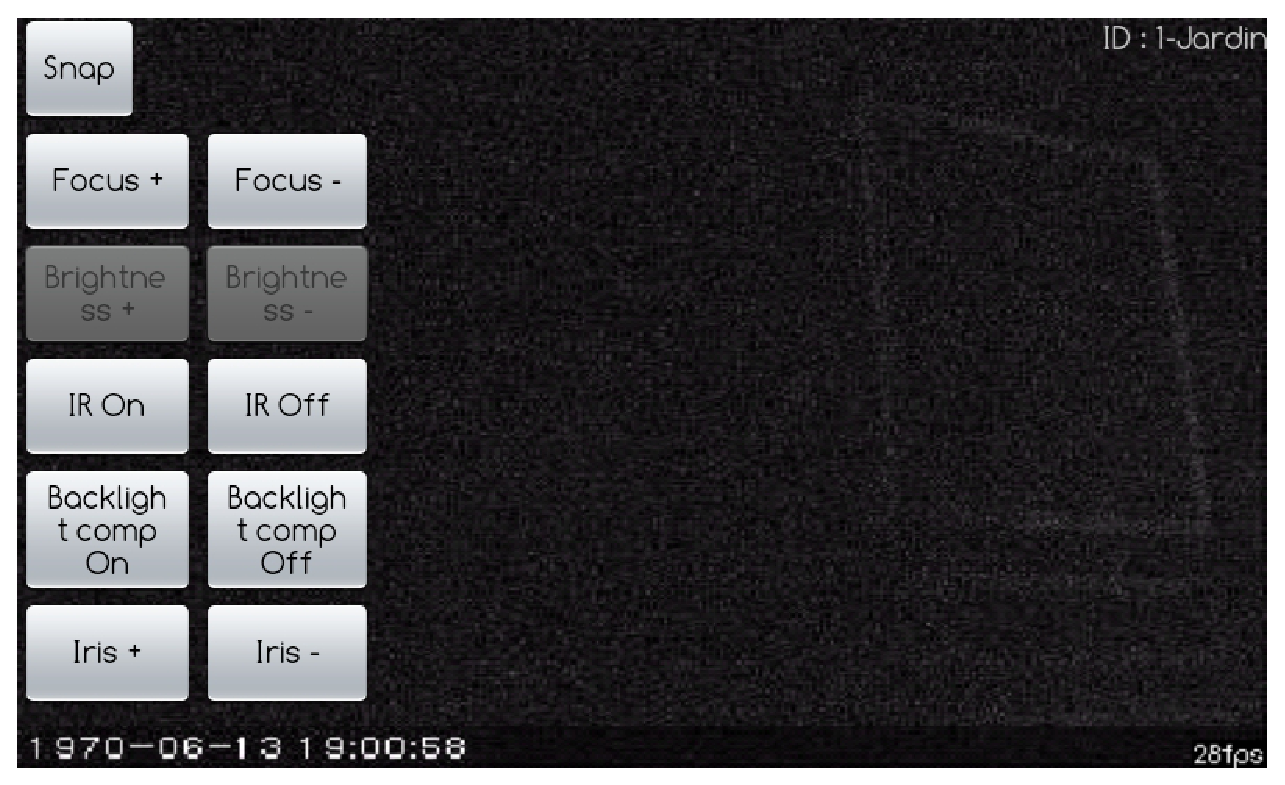
\includegraphics[scale=0.4]{Images/ctrl2.eps}
  \caption{Advance Controls}
\end{figure}  
\begin{itemize}
  \item \underline{Focus + / Focus - :} Augmenter ou diminuer la mise au
  point.
  \item \underline{Brightness + / Brightness - :} Augmenter ou diminuer la luminosité
  \item \underline{Iris + / Iris - :} Augmenter ou diminuer l'exposition.
  \item \underline{IR On / IR Off :} Activer ou desactiver le filtre
  anti-IR
  \item \underline{Backlight comp On / Backlight comp Off :} Activer ou
  desactiver la correction pour la surexposition a la lumiere.
\end{itemize}
Mais nous avons également offert la possibilité a l'utilisateur d'utiliser les
réglages automatique de la caméra toujours a partir du menu de l'activitée
\textit{Video}.
\begin{figure}[H]
  \label{ctrl2}
  \centering
   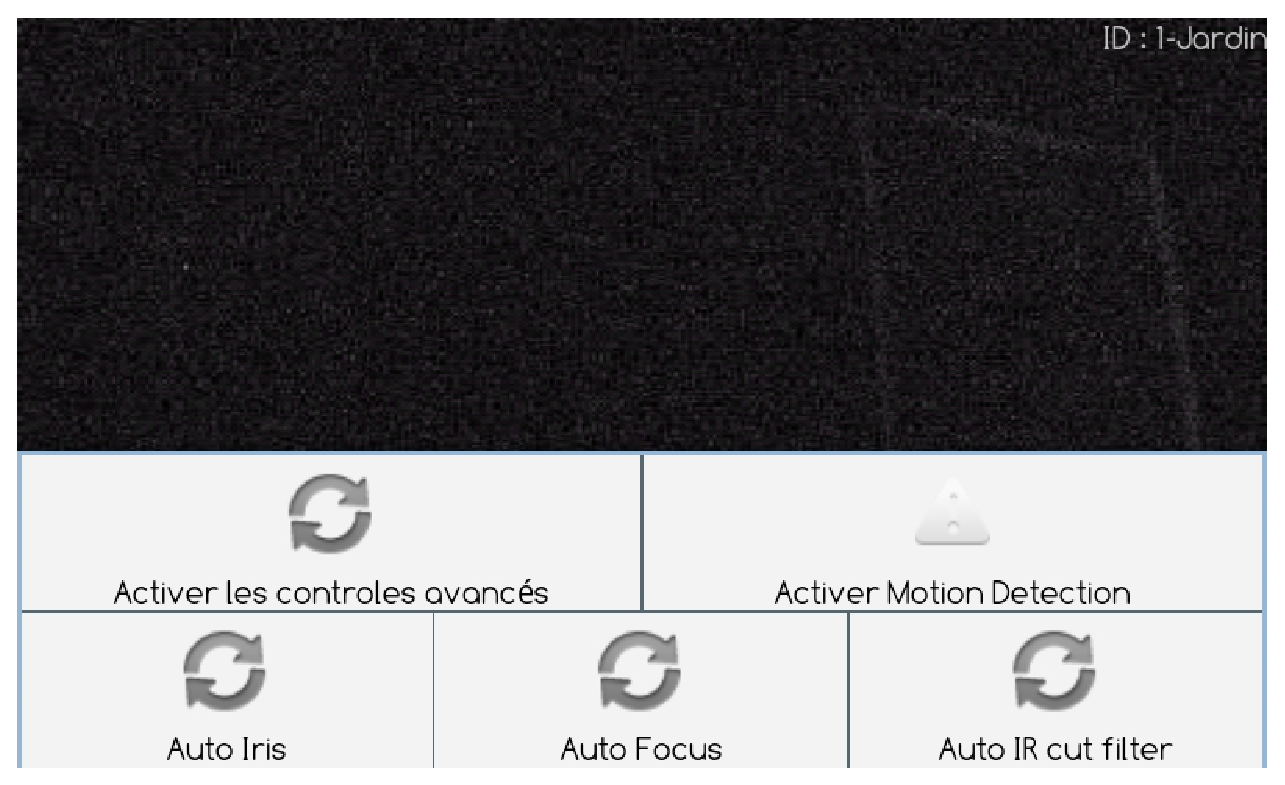
\includegraphics[scale=0.4]{Images/ctrl1.eps}
  \caption{Advance Controls}
\end{figure}  

\section{Détection de mouvements}
\subsection{Présentation}
La détéction de mouvement est une mécanisme utiliser pour detecter les
changements de position, et les mouvement d'objets ou d'indicidu dans une
zone couverte par un dispositif de video-surveillance.\newline
Selon une traduction de la definition de wikipedia\footnote{\label{MotionDetection}
http://en.wikipedia.org/wiki/Motion\_detection} : \newline
\begin{quotation}
`` Ceci peut être réalisé soit par des dispositifs mécaniques qui interagissent
physiquement avec la zone ou par des dispositifs électroniques qui permettent de
quantifier et mesurer les changements dans l'environnement donné.
Le mouvement peut être détecté par: son (capteurs acoustiques), l'opacité
(capteurs optiques et infrarouges et des processeurs d'images vidéo), le
géomagnétisme (capteurs magnétiques, magnétomètres), la réflexion de l'énergie
transmise (radar laser infrarouges, capteurs ultrasoniques, capteurs et radars
micro-ondes), induction électromagnétique (détecteurs à boucle inductive), et
les vibrations (triboélectrique, sismiques, et des capteurs d'inertie-switch). ``
\end{quotation}
\indent La caméra mise a notre disposition contient un service capable de
detecter les mouvements couvert par l'objectif ou limité a une zone
particuliere.\newline Nous avons souhaiter offrir a l'utilisateur la possibilité
de detecter les mouvements et d'en etre avertie en temps réel sur son telephone.
C'est pourquoi nous avons implémenté un service a l'écoute de chacune des
cameras afin de detecter les mouvements sans que l'application soit active.
\subsection{Utilisation de service Android}
Sous Android, les services sont des composants qui permettent l'execution de
fonctionnalités en arriere plan pendant une durée indeterminée meme lorsque les
activitées de l'application ne sont pas lancée.
Pour créer un service il faut dans un premier temps le declarer dans le fichier
\textit{AndroidManifest.xml} :\newline
\begin{lstlisting}
<application android:icon="@drawable/camera" android:label="@string/app_name">
	<activity <!-- activities list --> />
	<service android:name="MotionDetectionService" />
</application>
\end{lstlisting}
Puis en implémentant le service dans le fichier
\textit{MotionDetectionService.java}.
 Tout comme les activitées, les services ont
un cycle de vie :
\newpage
\begin{center}
\begin{figure}
   \label{serviceLifecycle}
  \centering
  \fbox{
  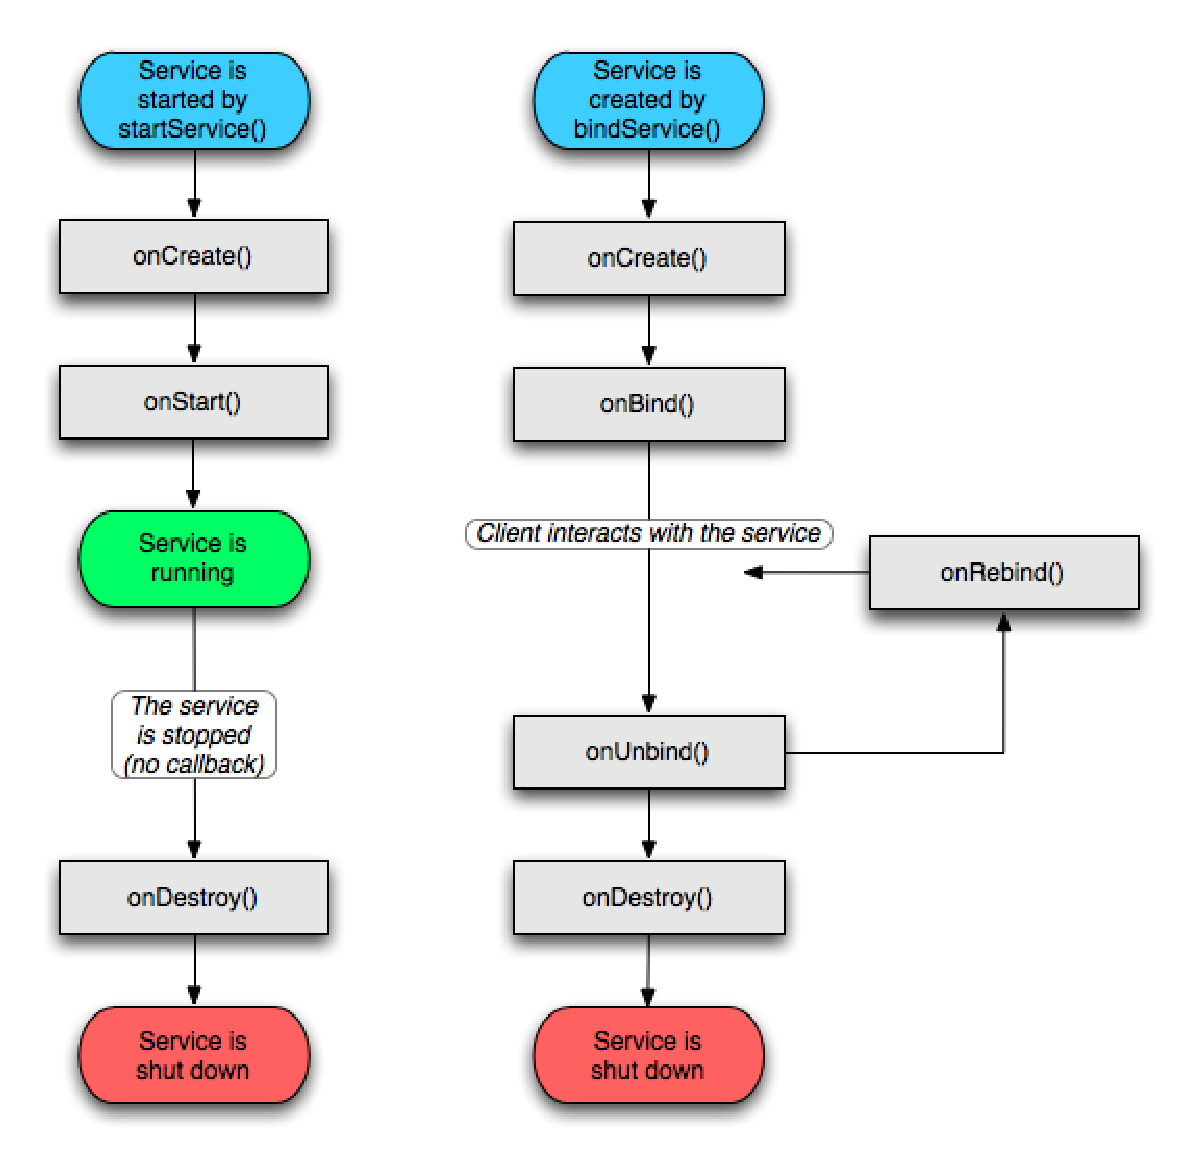
\includegraphics[scale=0.7]{Images/serviceLifecycle.eps}
  }
   \caption{Service Life Cycle \protect\footnotemark}
  \end{figure}
  \end{center}
\footnotetext{http://www.linuxtopia.org/online\_books/android/devguide/guide/topics/fundamentals.html}
\newpage

Ce shcema illustre la possibilité de contacter un service de deux manieres
differentes. La premiere (cycle de gauche) se limite a envoyer des insctuctions 
au service pour y declancher un traitement definit dans la fonction :
\begin{lstlisting}
@Override
public int onStartCommand(Intent intent, int flags, int startId){
/* work to do */
}
\end{lstlisting}
La seconde (cycle de droite) permet a une activitée de se lier a
un service afin de pouvoir utiliser toutes les méthodes public du
service.\newline
N'ayant pas besoin de communiquer autrement avec les services que pour leurs
demander d'effectuer un traitement, la premiere methode nous avons choisi
d'implémenter le 1er cycle.

\subsection{Activation du service}
Les caméras Axis peuvent gerer jusqu'a dix fenetre de detection de mouvement par
caméra simutanement. Pour ajouter une fenetre (avec les valeurs par defaut) il
suffit d'envoyer une requette \textit{HTTP GET} a l'adresse : 
\begin{lstlisting}
http://myserver/axis-cgi/operator/param.cgi?action=add&group=Motion&template=motion
\end{lstlisting}
Pour ajouter une fenetre defini par sa position sur l'ecran, il faut spécifier
explicitement la position de la fenetre :
\begin{lstlisting}
http://myserver/axis-cgi/operator/param.cgi?action=add&group=Motion&template=motion
&Motion.M.Top=500
&Motion.M.Bottom=7000
&Motion.M.Left=5000
&Motion.M.Right=8500
\end{lstlisting}
Chacune de ces requettes nous fournira le numero du groupe (de 0 a 9) associer a
la requete, nous permettant plus tard de recuperer le niveau de la detection.
La reponse est de la forme : 
\begin{lstlisting}
HTTP/1.0 200 OK\r\n
Content-Type: text/plain\r\n
\r\n
M<group number> OK\r\n
\end{lstlisting}
Pour selectionner la fenetre a detecter, nous avons implementer un nouveau
composant graphique appelé \textit{drawRectOnTouchView} dont la fonction est de
dessiner un rectangle et de recuperer la position de la fenetre a partir d'un
clique de l'utilisateur.
\subsubsection{drawRectOnTouchView}
Comme pour le lecteur \textit{mjpeg}, l'implémentation d'un nouveau composant
graphique se fait en etendant la classe \textit{View}. Dans une premier temps il
faut definir les constructeurs (Création de la surface sur laquel dessiner,
definition des couleures, \ldots). Puis il est necessaire de surcharger la
methode :
\begin{lstlisting}
@Override
protected void onDraw(Canvas canvas)
\end{lstlisting}
afin de dessiner le composant. Dans notre utilisation, nous souhaitons dessiner
dynamiquent un dessin en fonction des interactions fournient par l'utilisateur.
Android nous propose de surcharger une fonction qui est appeler lors de chaque
interaction avec le composant appelé : 
\begin{lstlisting}
@Override
public boolean onTouchEvent(MotionEvent event)
\end{lstlisting}
Grace a cette fonction, nous allons dessiner un rectangle qui suivra le doigt de
l'utilisateur jusqu'a ce qu'il relache la pression de l'écran.
Précédement nous avons présenté les actions definie par les
\textit{MotionEvent}. Nous allons egalement a nouveau utiliser ces interactions
pour definir le comportement de notre composants :
\begin{lstlisting}[caption={Draw Rectangle Component}] 
@Override
public boolean onTouchEvent(MotionEvent event) {
	float x = event.getX();
	float y = event.getY();
	switch (event.getAction()) {
	case MotionEvent.ACTION_DOWN:
	    start.set(x, y);
	    isDraw = false;
	    break;
	case MotionEvent.ACTION_MOVE:
	    end.set(x, y);
	    isDraw = false;
	    invalidate();
	    break;
	case MotionEvent.ACTION_UP:
	    end.set(x, y);
	    isDraw = true;
	    invalidate();
	    break;
	}
	return true;
    }
    
@Override
    protected void onDraw(Canvas canvas) {
	canvas.drawColor(Color.TRANSPARENT);
	canvas.drawLine(start.x, end.y, end.x, end.y, mPaint);
	canvas.drawLine(end.x, start.y, end.x, end.y, mPaint);
	canvas.drawLine(start.x, start.y, start.x, end.y, mPaint);
	canvas.drawLine(start.x, start.y, end.x, start.y, mPaint);
    }
\end{lstlisting}
Lors de l'appuie sur l'ecran, nous sauvegardons les coordonnées du point, puis
dès le deplacement du doigt de l'utilisateur, on commence a tracer le rectangle.
Enfin lorsque l'utilisateur releve son doigt, on sauvegarde la position du
point, puis on signal que le dessin est dessiné a l'aide du flag
\textit{isDraw}. La fonction \textit{onDraw} nous permet de dessiner les aretes
du rectangle a partir des coordonnées sauvegardées.\newline
\indent Enfin en affectant la couleur ``transparente'' au fond du composant, on
peut le superposer au dessus d'une vue \textit{mjpeg} pour dessiner un rectangle
sur notre video.\newline
\newline\indent Une fois la detection activée aupres de la caméra, nous pouvons
demarrer notre service en lui indiquant le groupe fournis par la caméra.

\subsection{Detection et Signalisation}
Dans cette partie nous allons etudier le comportement du service.
La detection de mouvement aupres des caméra \textit{Axis} se fait au travers de
la requete GET: 
\begin{lstlisting}
http://myserver/axis-cgi/motion/motiondata.cgi?group=<group number>
\end{lstlisting}
Dans le resultat de cette requete, nous nous interessons a la valeure du niveau
de detection. Si celui ci depasse le seuil defini dans les parametre
utilisateur, le service declanche une notification sous forme de vibration du
telephone.\newline
\begin{lstlisting}
HTTP/1.0 200 OK\r\n
Content-Type: multipart/x-mixed-replace;boundary=axismdb\r\n\r\n
--axismdb\r\n
Content-Type:text/plain\r\n\r\n
group=0;level=28;threshold=45;\r\n
group=1;level=43;threshold=25;\r\n
--axismdb\r\n
Content-Type:text/plain\r\n\r\n
group=0;level=54;threshold=45;\r\n
group=1;level=38;threshold=25;\r\n
--axismdb\r\n
Content-Type:text/plain\r\n\r\n
group=0;level=49;threshold=45;\r\n
group=1;level=19;threshold=25;\r\n
--axismdb\r\n
 .
 .
 . 
\end{lstlisting}
Exemple tiré de la documentation de la caméra dans la partie
\textit{5.4.5 Get the Motion Detection
level\footnote{\label{MotionDetectionDoc}
http://www.axis.com/techsup/cam\_servers/dev/cam\_http\_api\_2.php\#api\_blocks\_motion\_get\_md\_level}.}
\newline\indent
Chaque demande de detection de mouvement aupres d'une caméra cré une
notification ``en cours'' dans la barre de status du telephone.
Ainsi l'utilisateur peut acceder facilement et rapidement a la caméra dont il
surveille les mouvement.


\section{Gestion des préférences}
\subsection{Import / Export}

\subsection{Shared Preferences}

\section{Multilangues, Interface et Partage}

\section{Tests}

\section{Optimisations / Extensions futures}
\subsection{Retransmission du signal audio}
\subsection{Enregistrement vidéo}
\subsection{Edition des fenêtres de détection  de mouvement}
\subsection{Ajout d'evénements suite à la détection (mail / snapshot)}
\subsection{Compte utilisateur}
\clearpage
